\documentclass[10pt,a4paper]{article}
\usepackage[utf8x]{inputenc}
\usepackage[danish]{babel}
\usepackage{amsmath}
\usepackage{mathtools}
\usepackage{framed}
\usepackage{amsfonts}
%\usepackage{epstopdf}
%\usepackage{hyperref}
\usepackage{todonotes}
\usepackage{subfig}
\usepackage{float}
\usepackage{amssymb}
\setlength{\parindent}{0pt}
\usepackage{graphicx}
\usepackage{fullpage}
\DeclarePairedDelimiter\ceil{\lceil}{\rceil}
\DeclarePairedDelimiter\floor{\lfloor}{\rfloor}
\newcount\colveccount
\newcommand*\colvec[1]{
        \global\colveccount#1
        \begin{pmatrix}
        \colvecnext
}
\def\colvecnext#1{
        #1
        \global\advance\colveccount-1
        \ifnum\colveccount>0
                \\
                \expandafter\colvecnext
        \else
                \end{pmatrix}
        \fi
}

\title{Exercise 3: Clustering}
\author{Group 2: Keerthikan Ratnarajah \& Mikael Westermann}


\begin{document}
\maketitle
\section{K - means clustering}
Clustering is the task of grouping a set of data points in such
a way that data points in the same group (called a cluster)
are more similar (in some sense or another) to each other
than to those in other groups (clusters).
The clustering is done by minimizing  the sum of squared distances
between each data point and their corrensponding cluster centroid. \\

In this exercise, the distance metric is Euclidean distance
in 324-dimensional space corresponding to pixel intensities of
the each hand written digit.
The digits were preprocessed by gaussian smoothing with smoothing parameter
\(\sigma=1.6\).

The number of clusters needed in k-means clustering is determined by the user.
It usually depends on how the data points are distributed.
Choosing a large number of clusters will result in a reduced
squared distance, and indeally zero as each data point gets it own cluster.
The optimal choice of k will consist of having a balance between having the
data compressed as possible, and still retain a decent amount of accuracy.
More fomally, the goal is to partition the data into k clusters in order to minimze the total
within cluster sum of squares. Here, the elbow method might become handy. \\

In this exercise, attention was given especially to run times of
the k-means clustering, because, as previous exercises have shown,
applying k-NN to the raw data sets
takes several minutes, and a reduction based on kmeans clustering
would be welcome.

\begin{figure}[H]
\centering
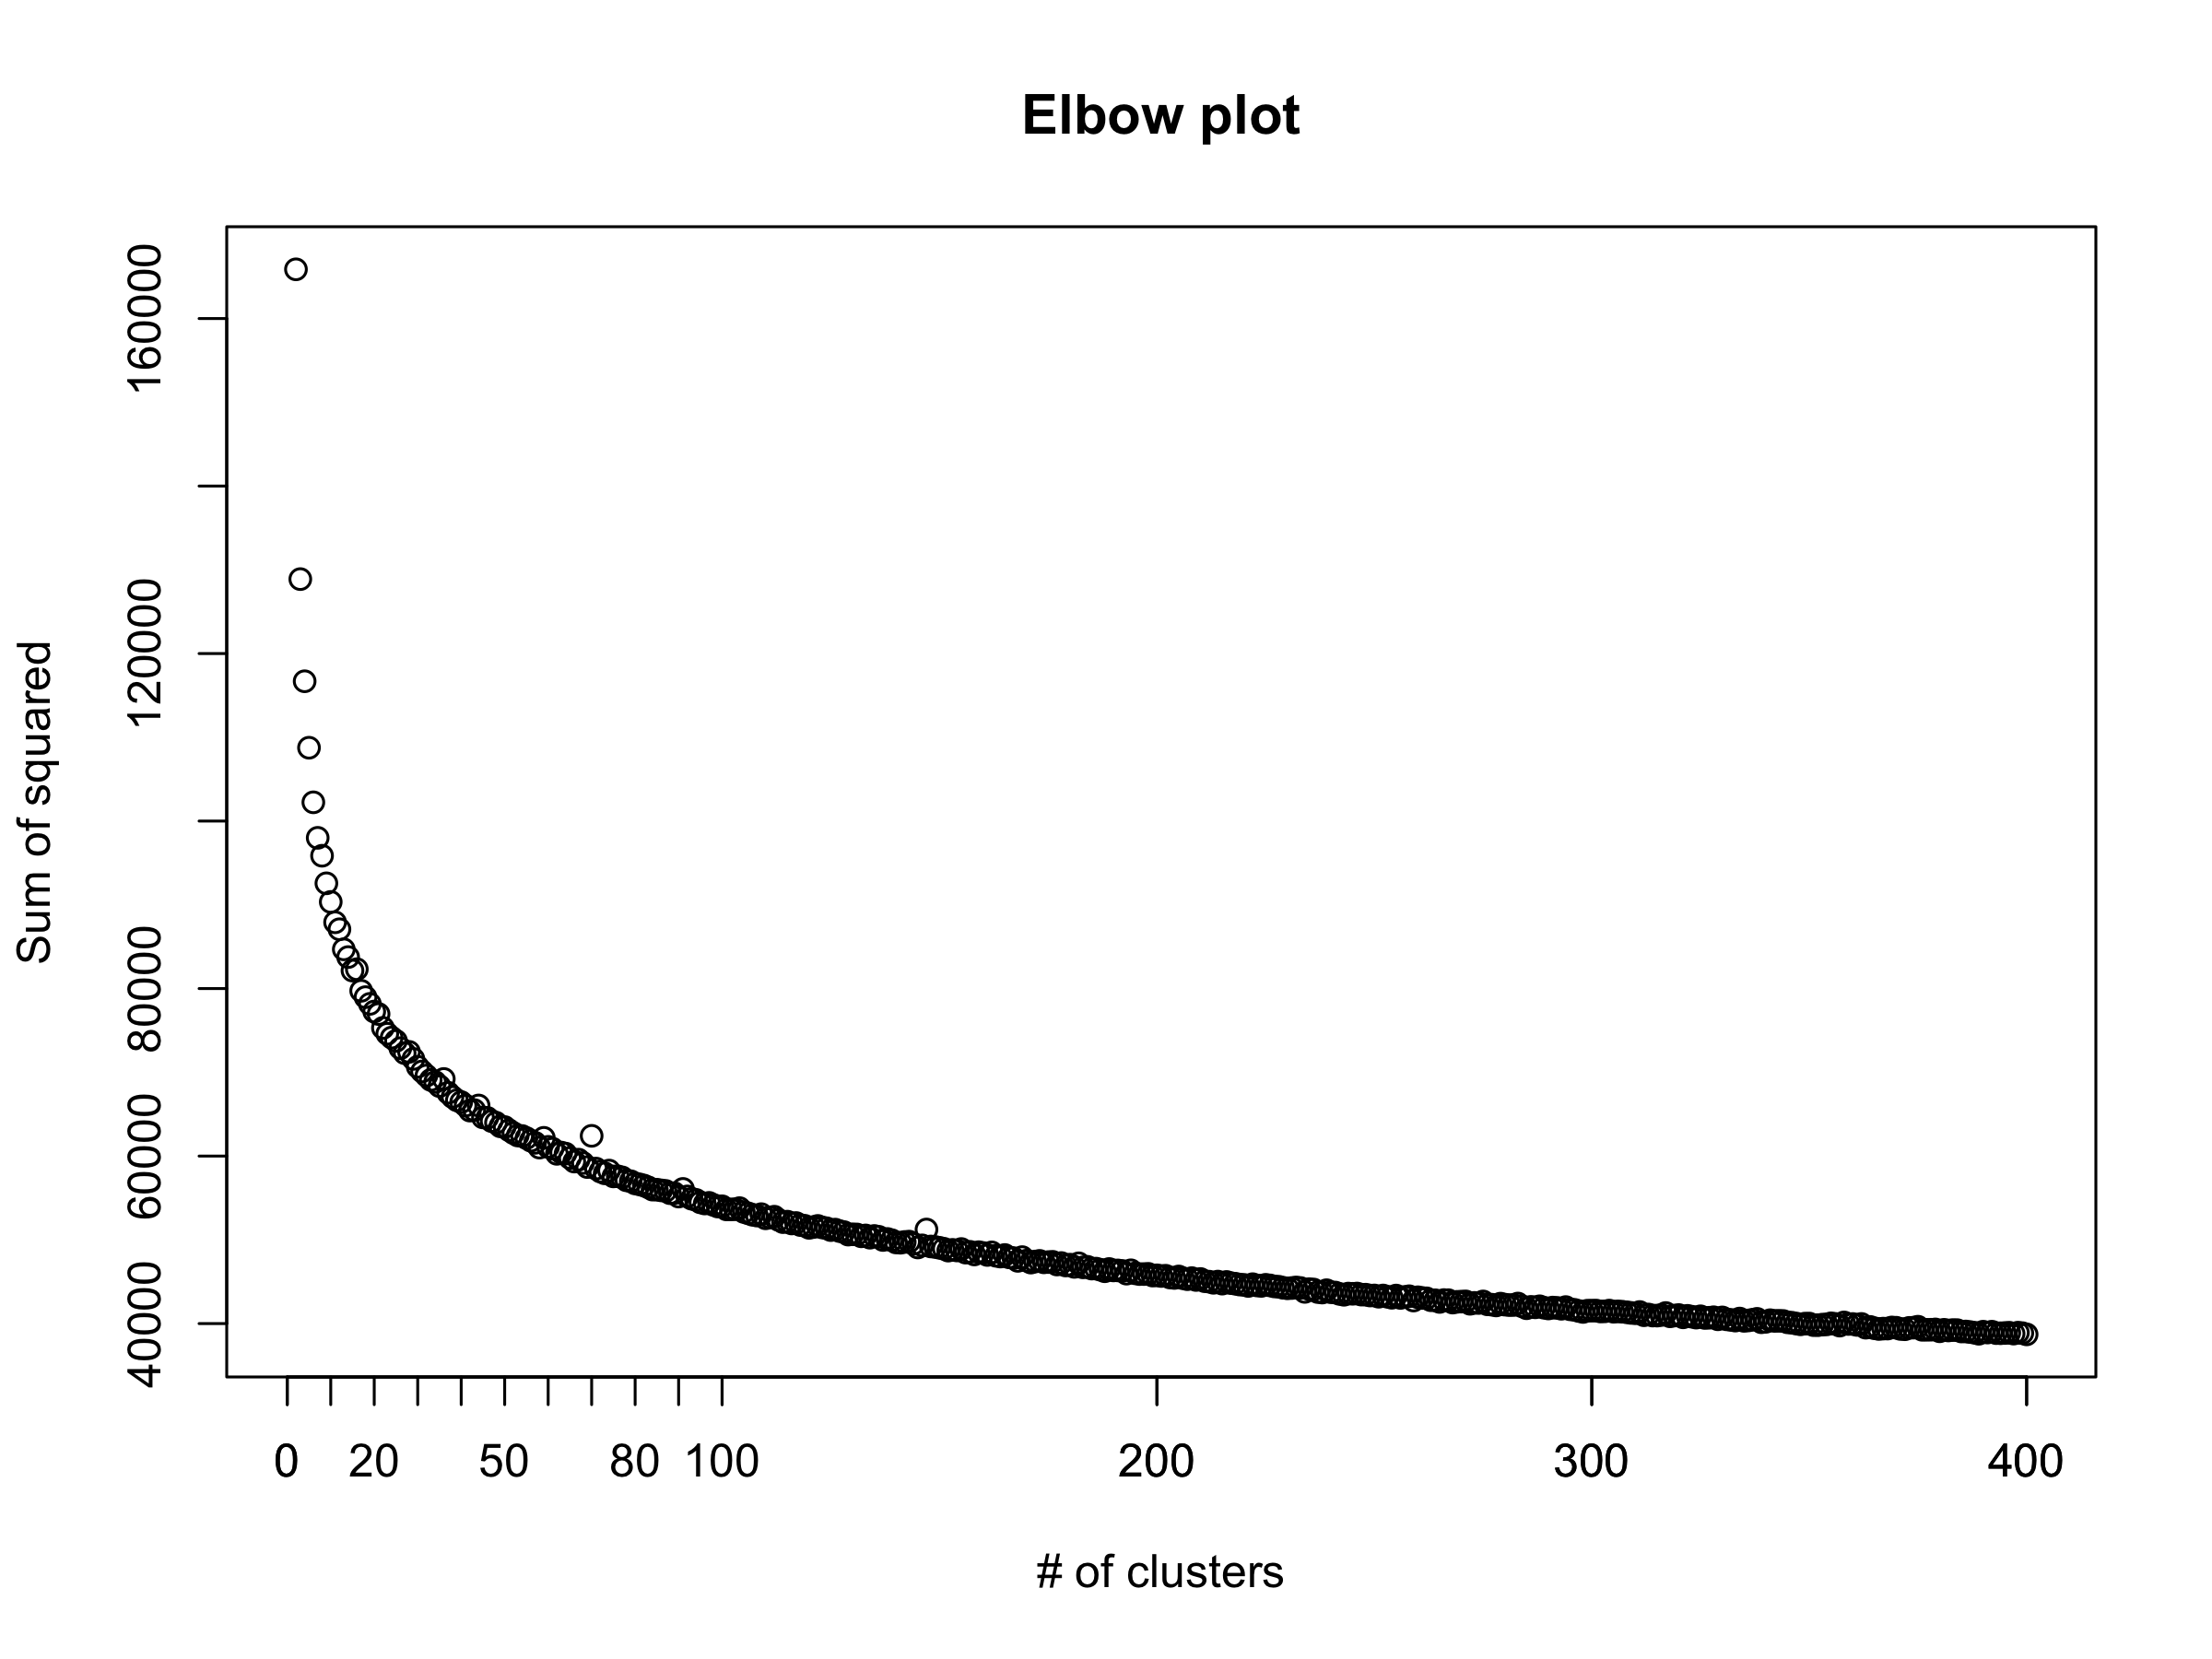
\includegraphics[width = 0.7\textwidth]{compl_elbow.png}
\caption{Sum of squared distances vs. number of clusters plot}
\label{fig:elbow}
\end{figure}

To find the optimal kmeans clustering, figure \ref{fig:elbow} was used to determine
what number of clusters would provide an optimal Total within sum of squared without having too
many cluster.  This is found by locating the elbow point of the graph, which lies around 30. 

Figures \ref{fig:0},\ref{fig:1}, \ref{fig:2},\ref{fig:3}, \ref{fig:4},\ref{fig:5}, \ref{fig:7},\ref{fig:8} and \ref{fig:9}, show how each digit is clustered along
the first two component axes of a post-processing PCA.
Some clustering tendency can be seen already from the firs two components,
but clearly, more components are required to reflect the clustering of the algorithm.
Each of the digits were clustered seperately from the other digits
which shows some form of overlap between each cluster.
Some of the  cluster may contain information about multiple digits
which figure \ref{fig:complete} shows, and thus the classes are not clearly
defined using this amount of clusters either.

\begin{figure}[H]
 		\centering
 		\subfloat[Class distribution within each cluster]{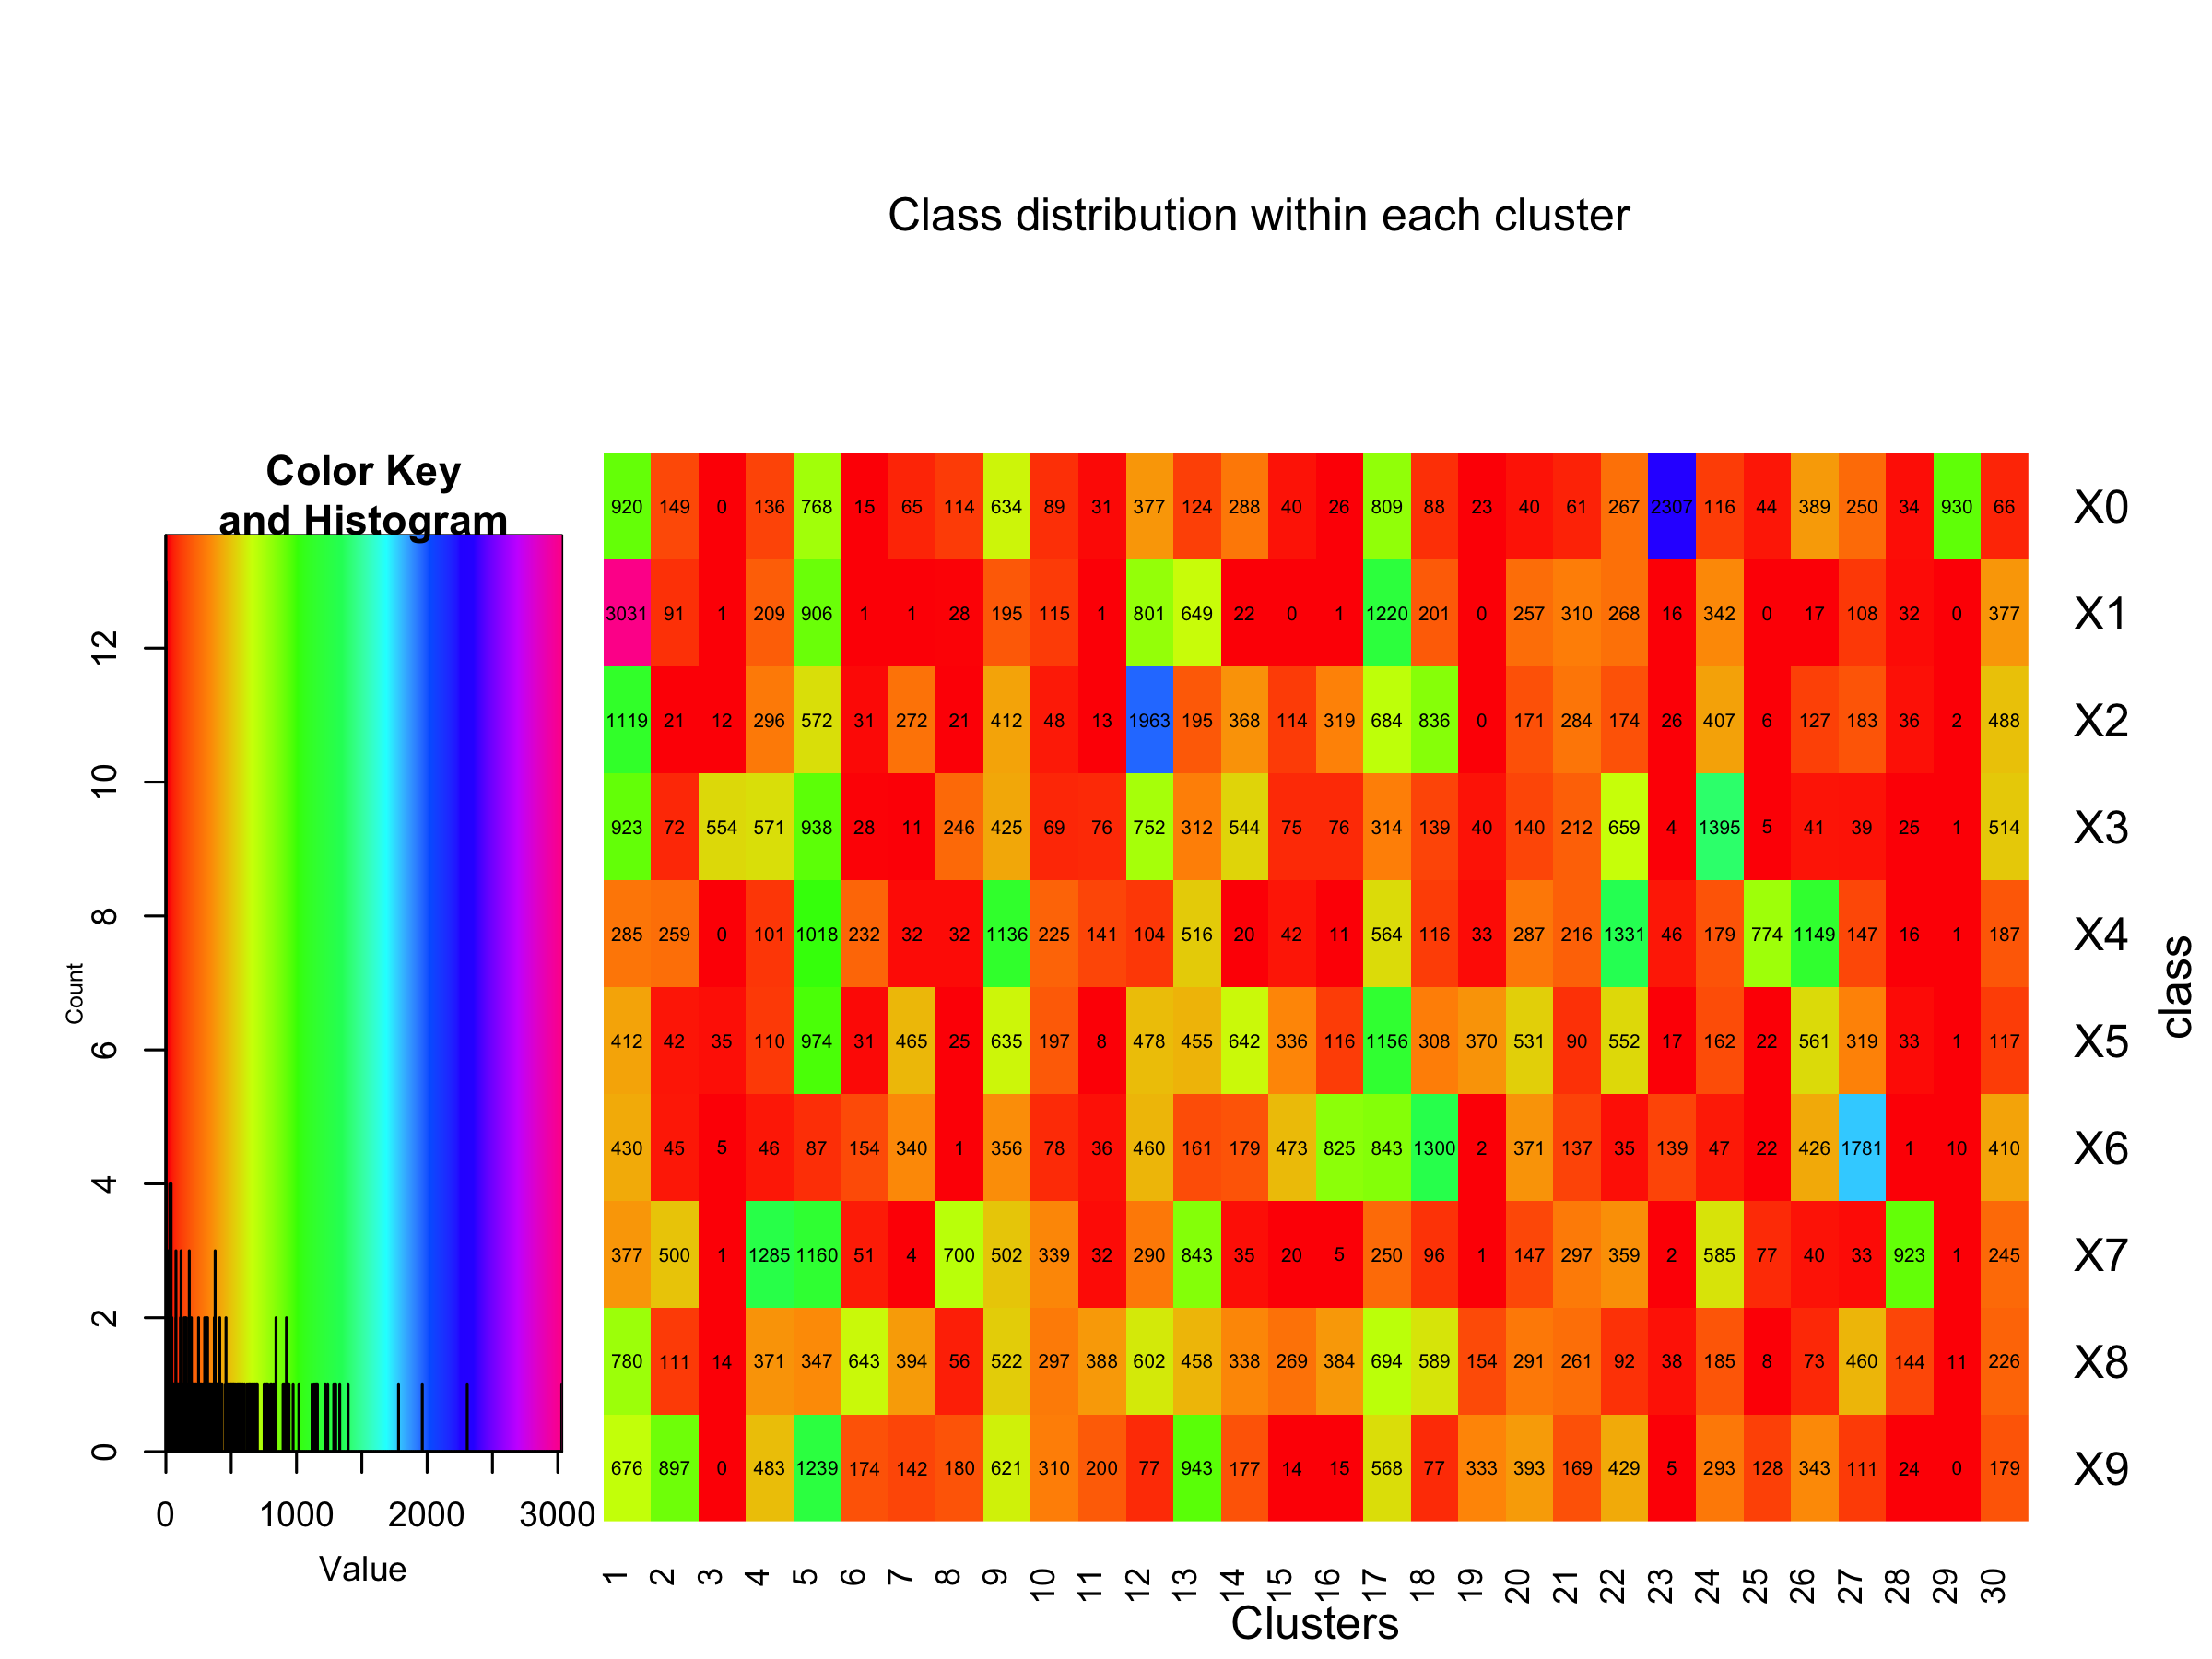
\includegraphics[width = 0.7\textwidth]{heatmap_comple.png}\label{fig:complete}} 

  		\subfloat[Clustering data consisting of digit 0]{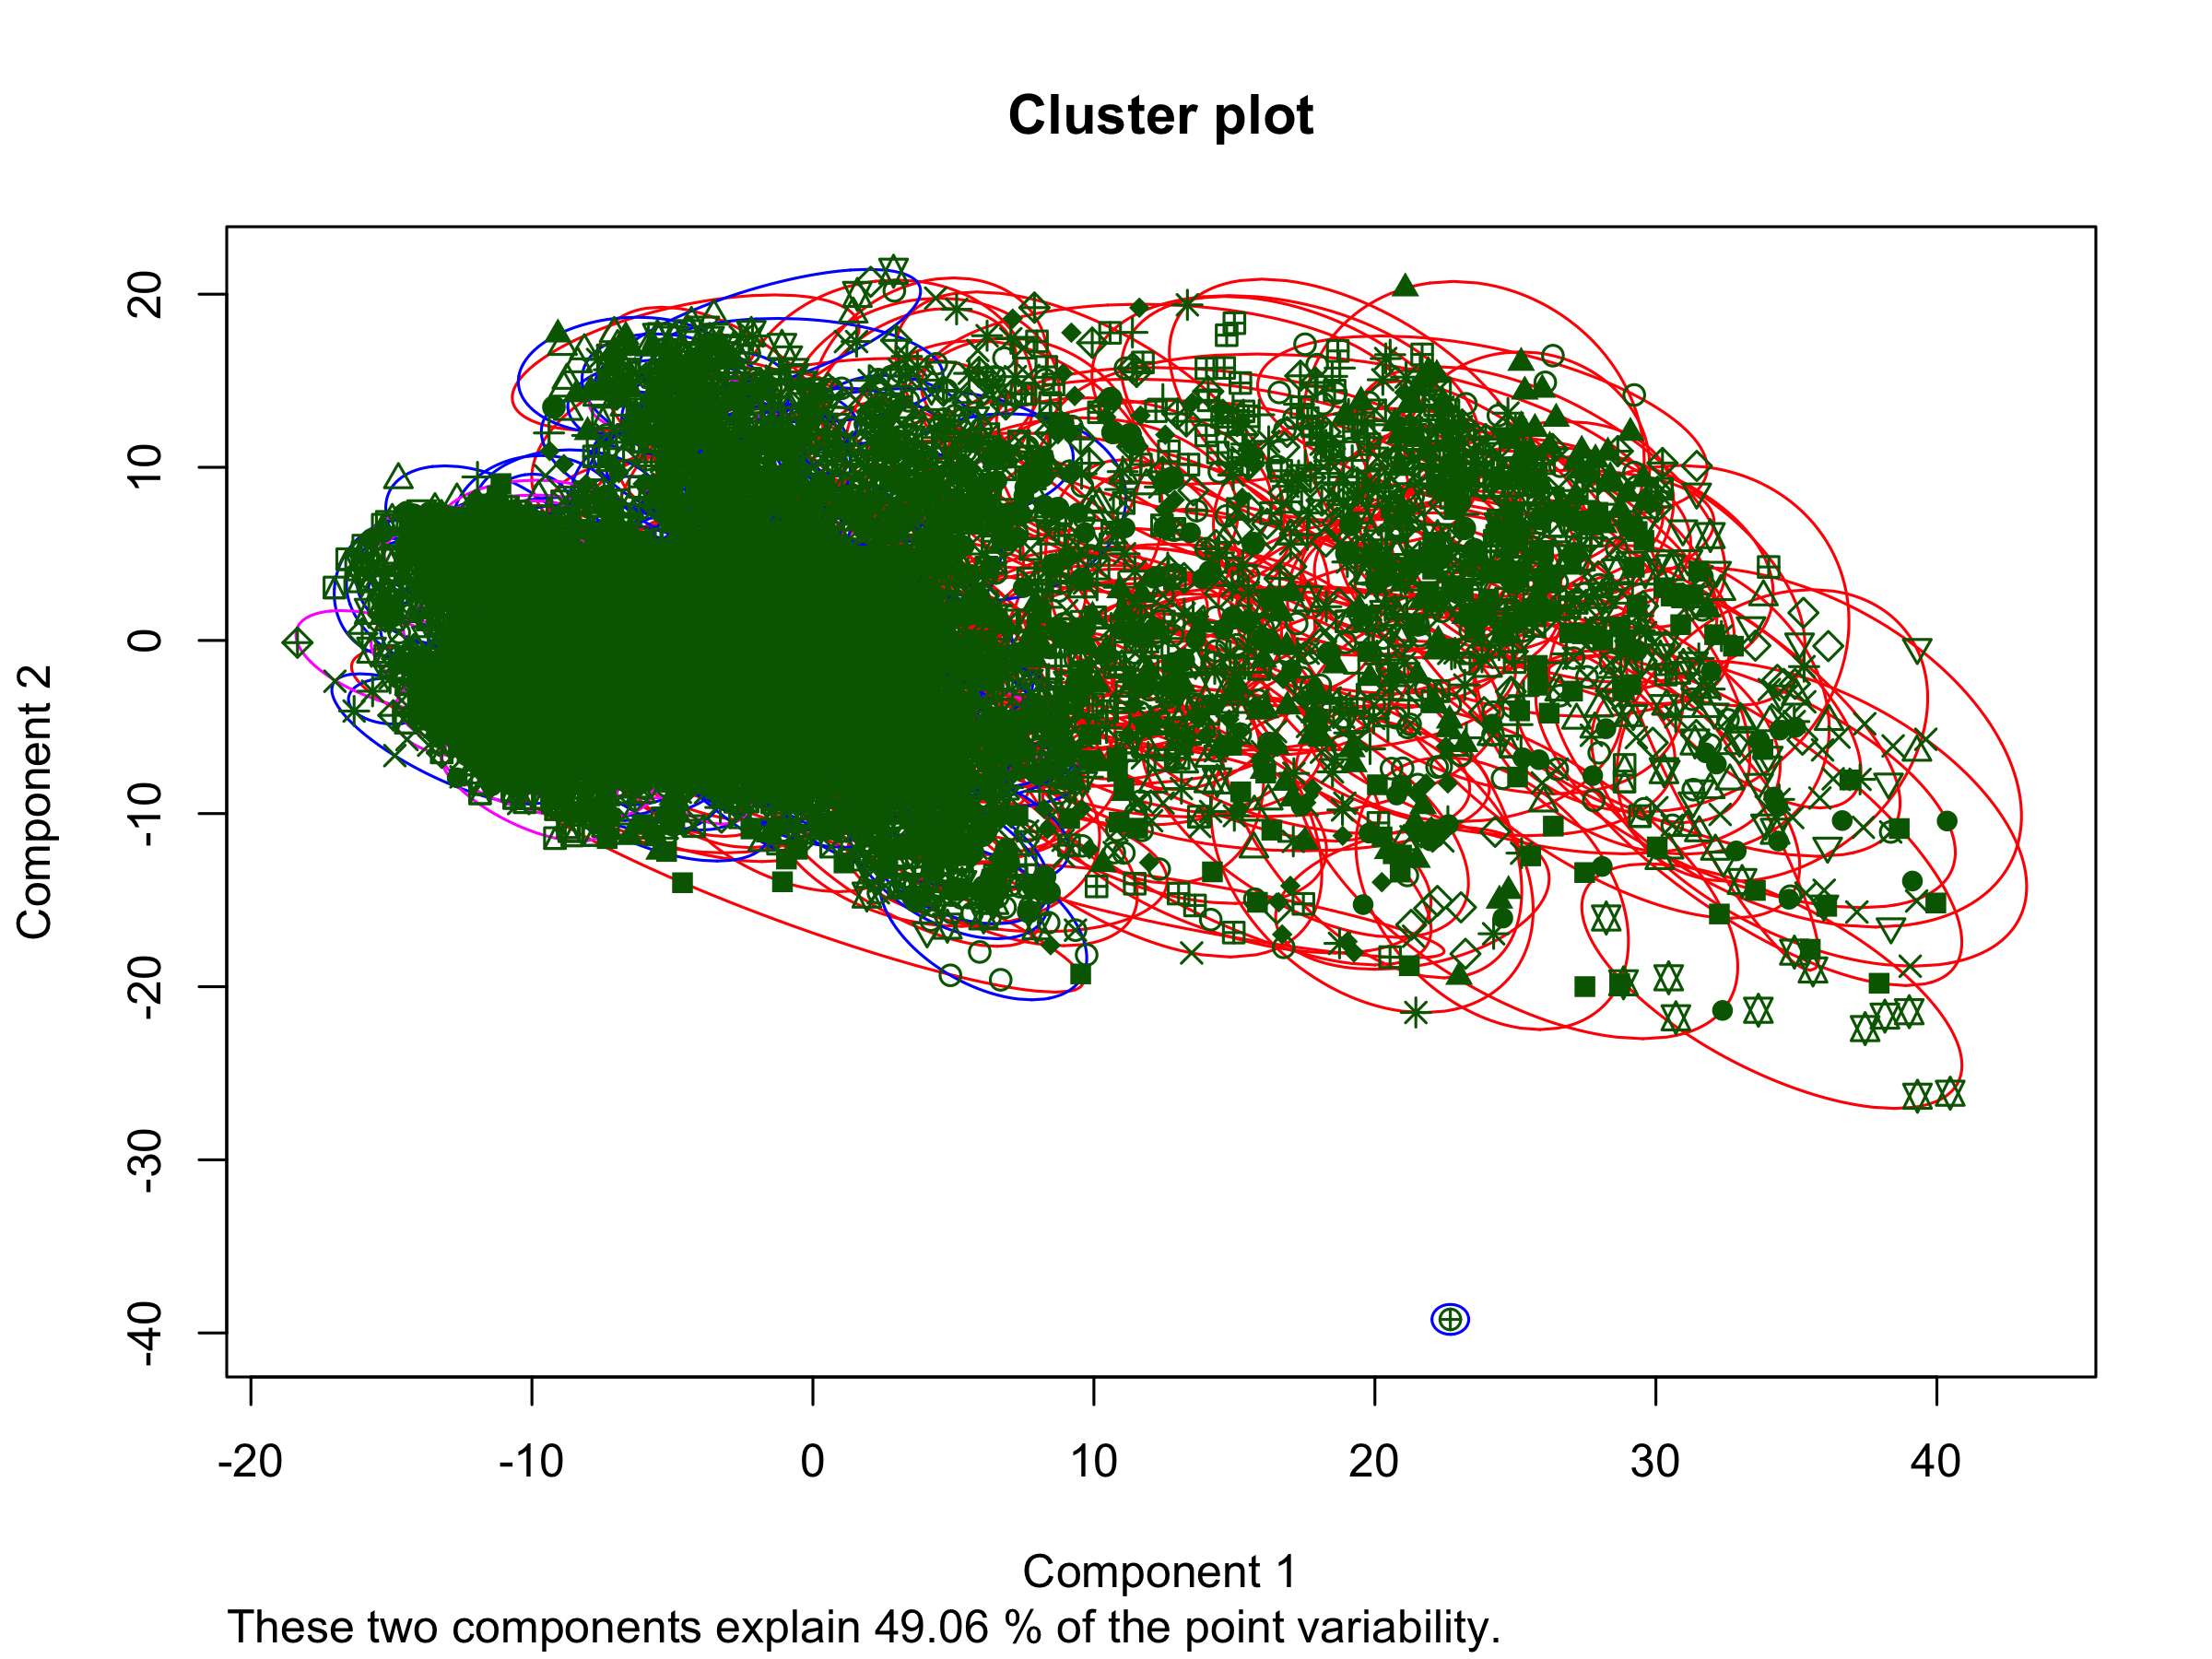
\includegraphics[width = 0.2\textwidth]{clusplot_0.png}\label{fig:0}}\hspace{1em}
%  		
  		\subfloat[Clustering data consisting of digit 1]{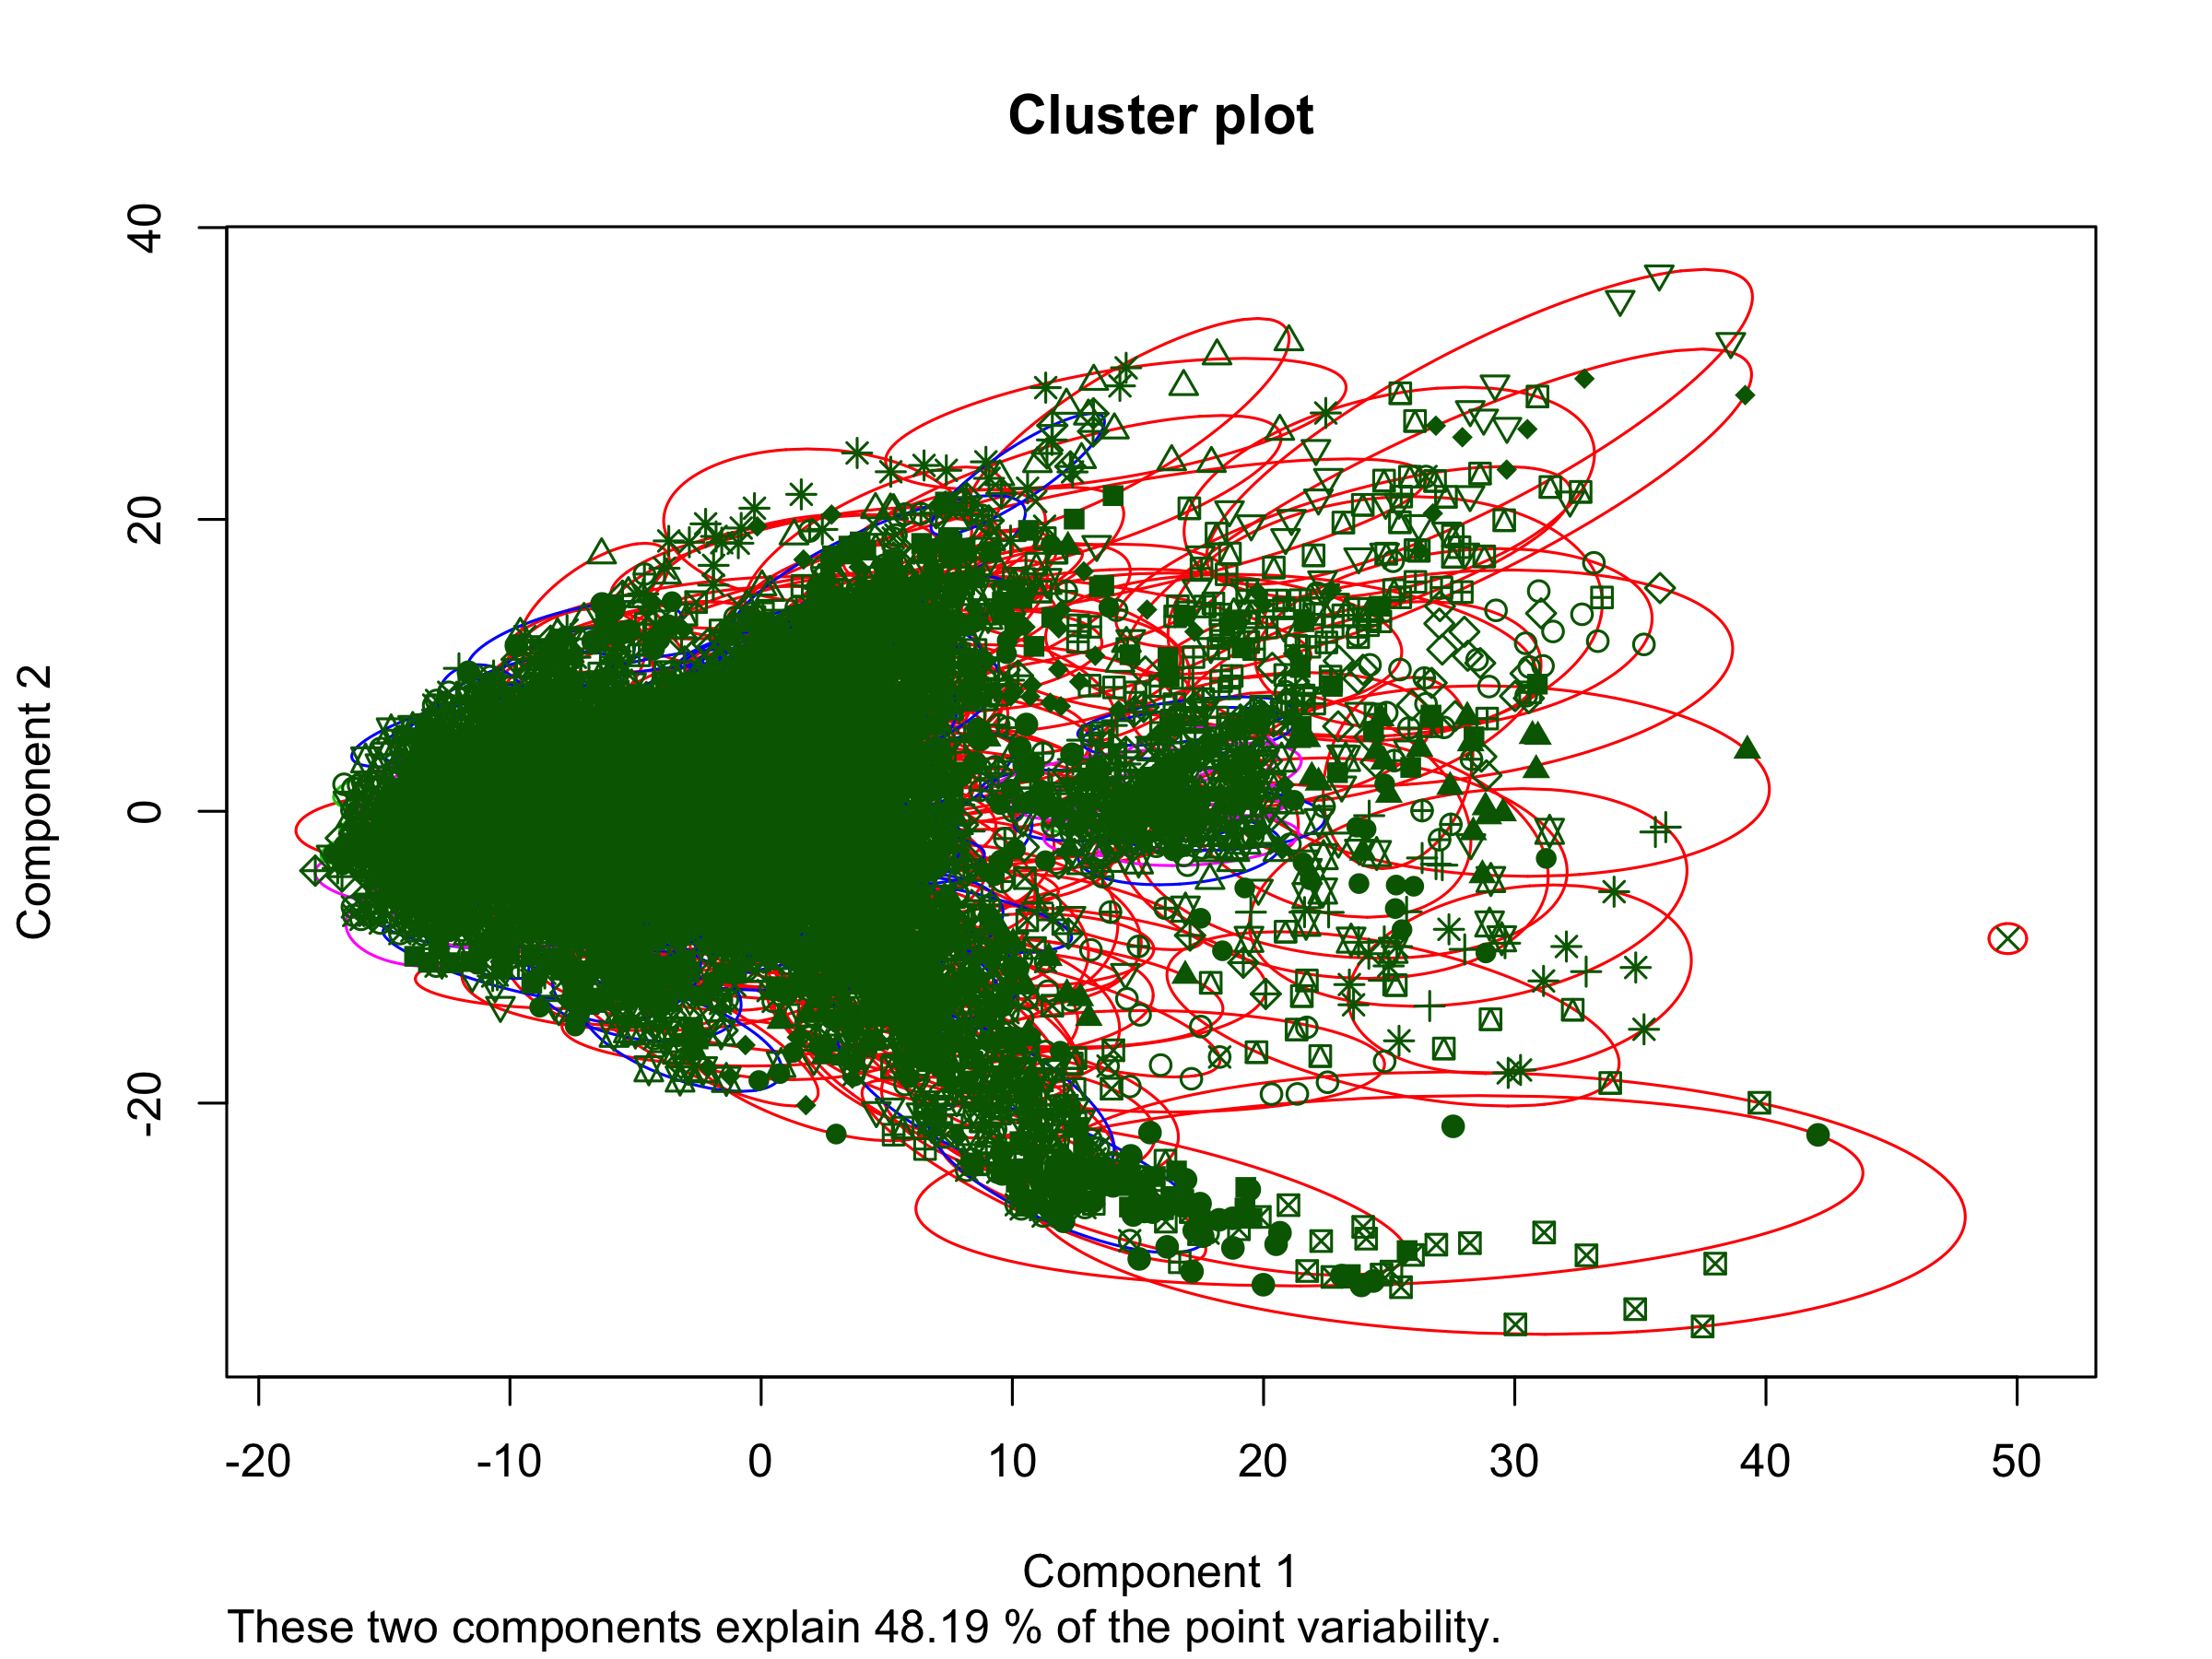
\includegraphics[width = 0.2\textwidth]{clusplot_1.png}\label{fig:1}}
%
  		\subfloat[Clustering data consisting of digit 2]{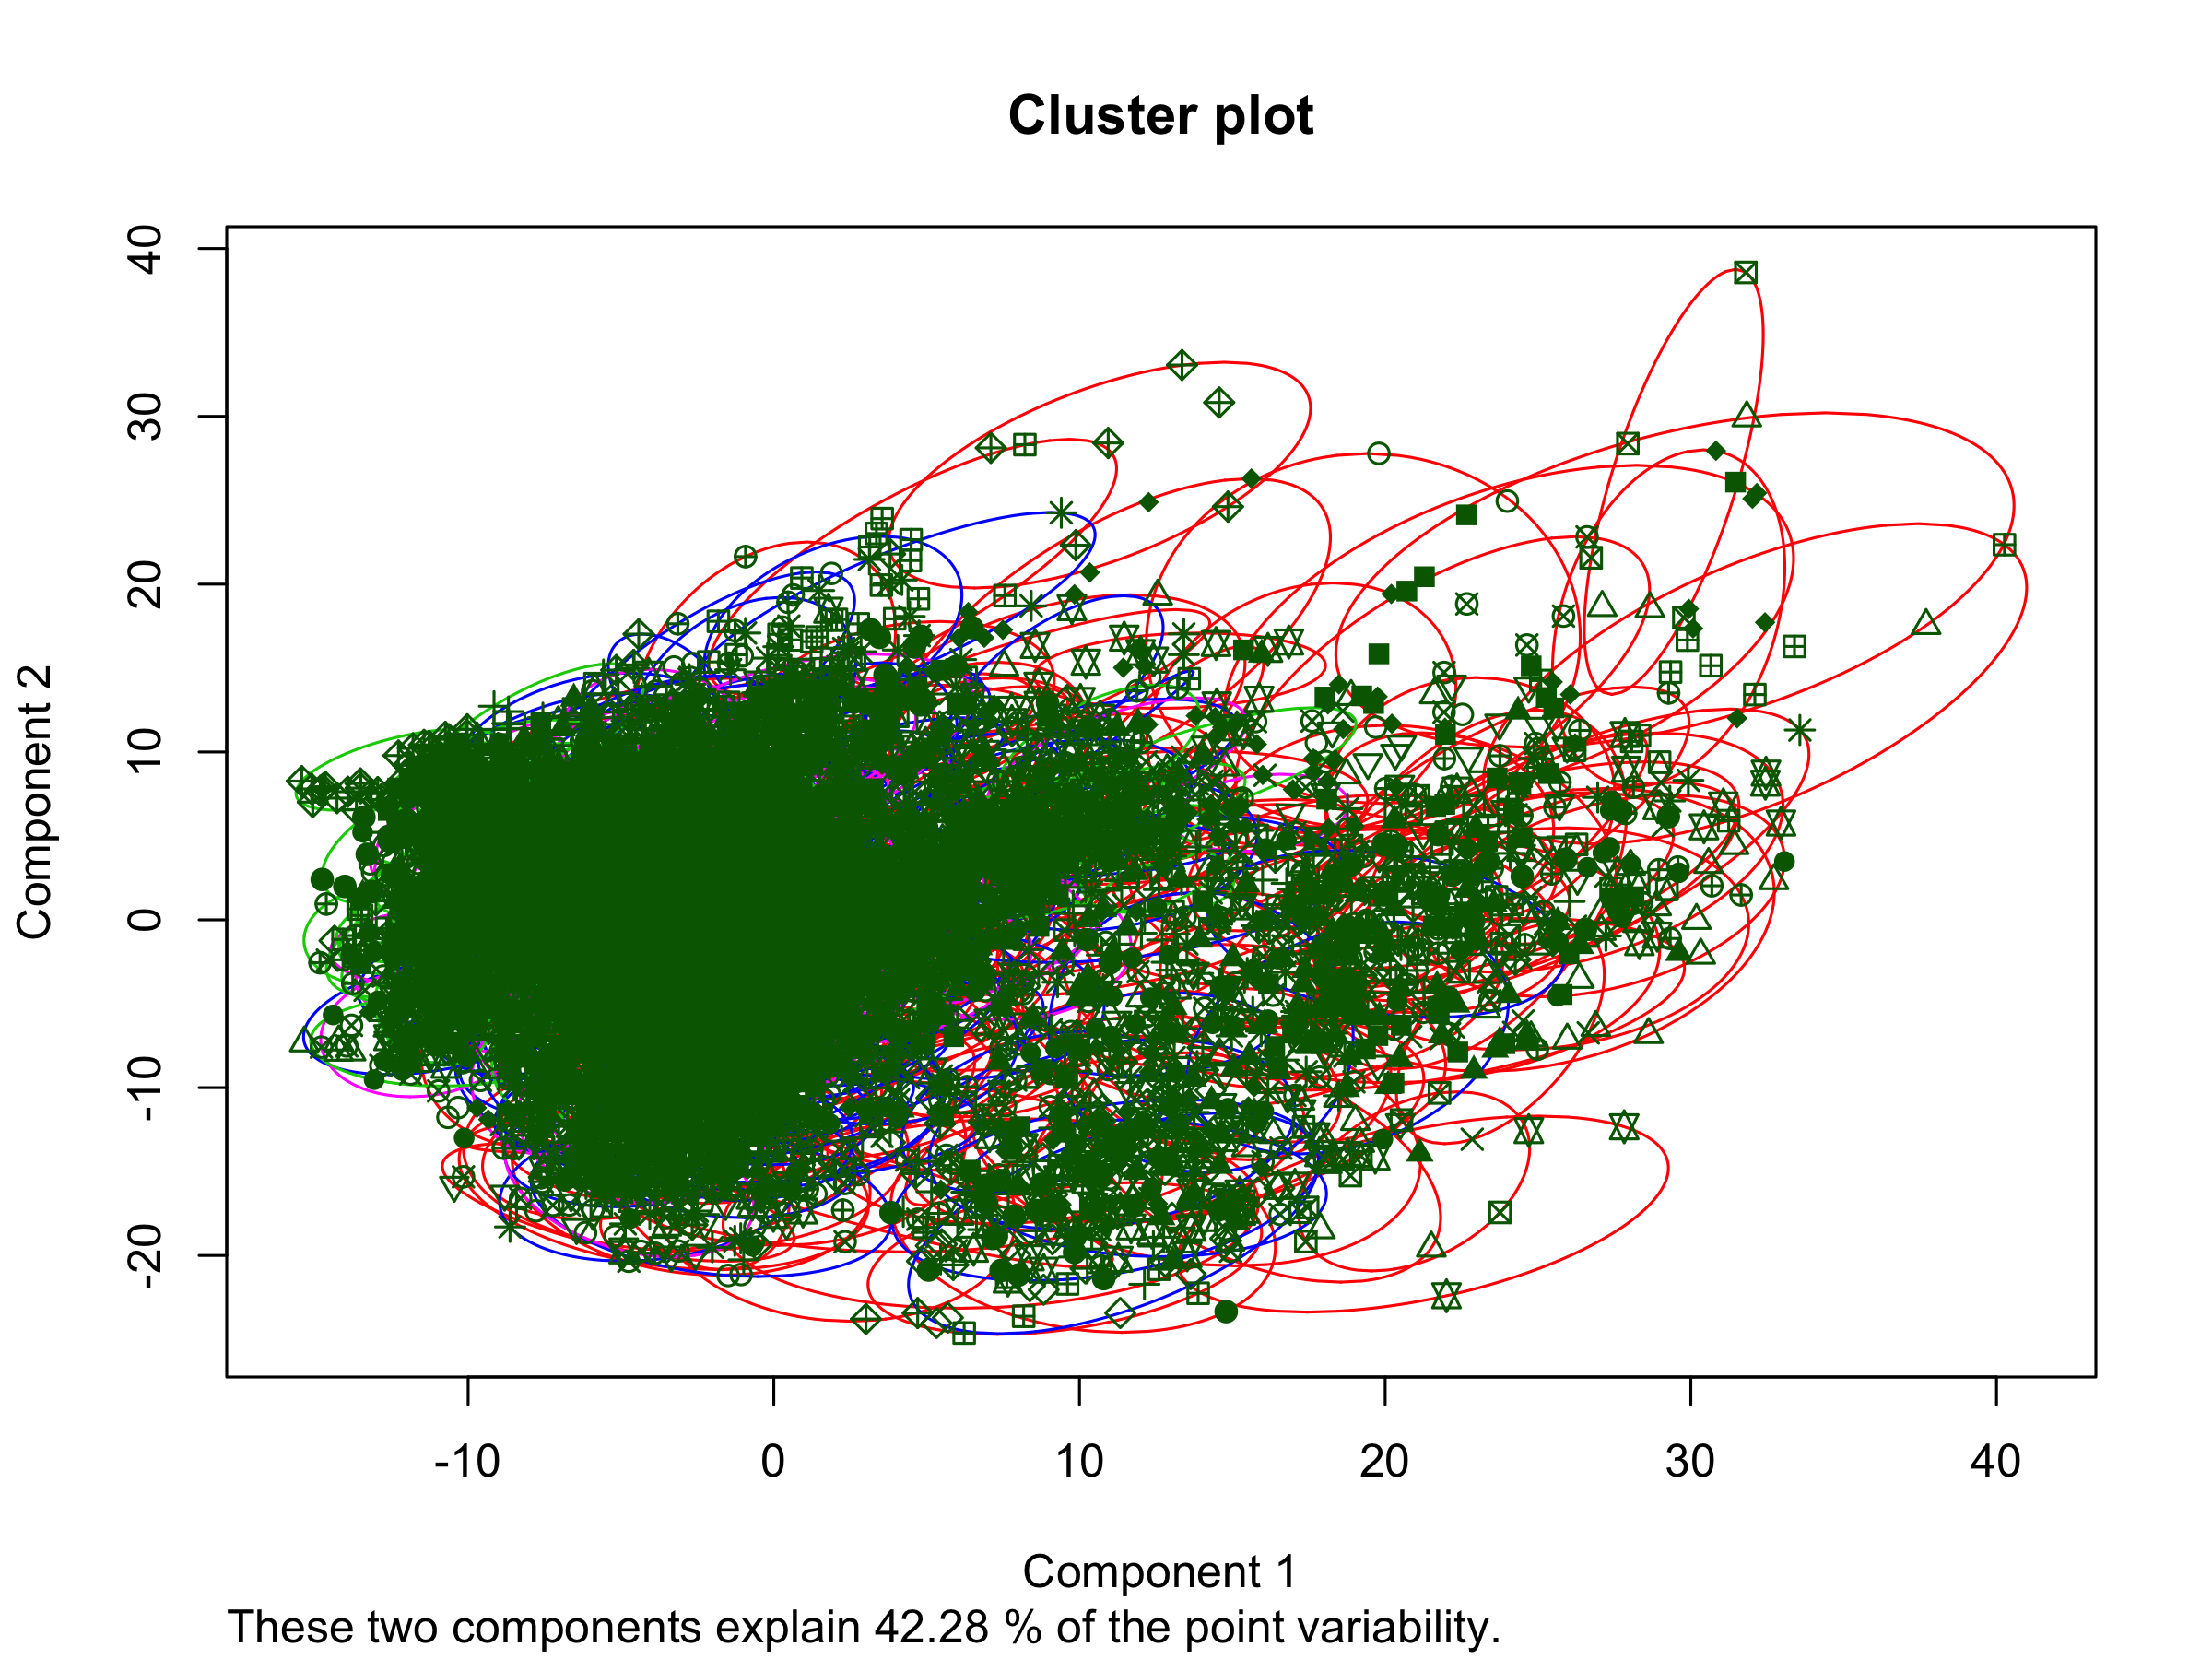
\includegraphics[width = 0.2\textwidth]{clusplot_2.png}\label{fig:2}}
%  		
  		\subfloat[Clustering data consisting of digit 3]{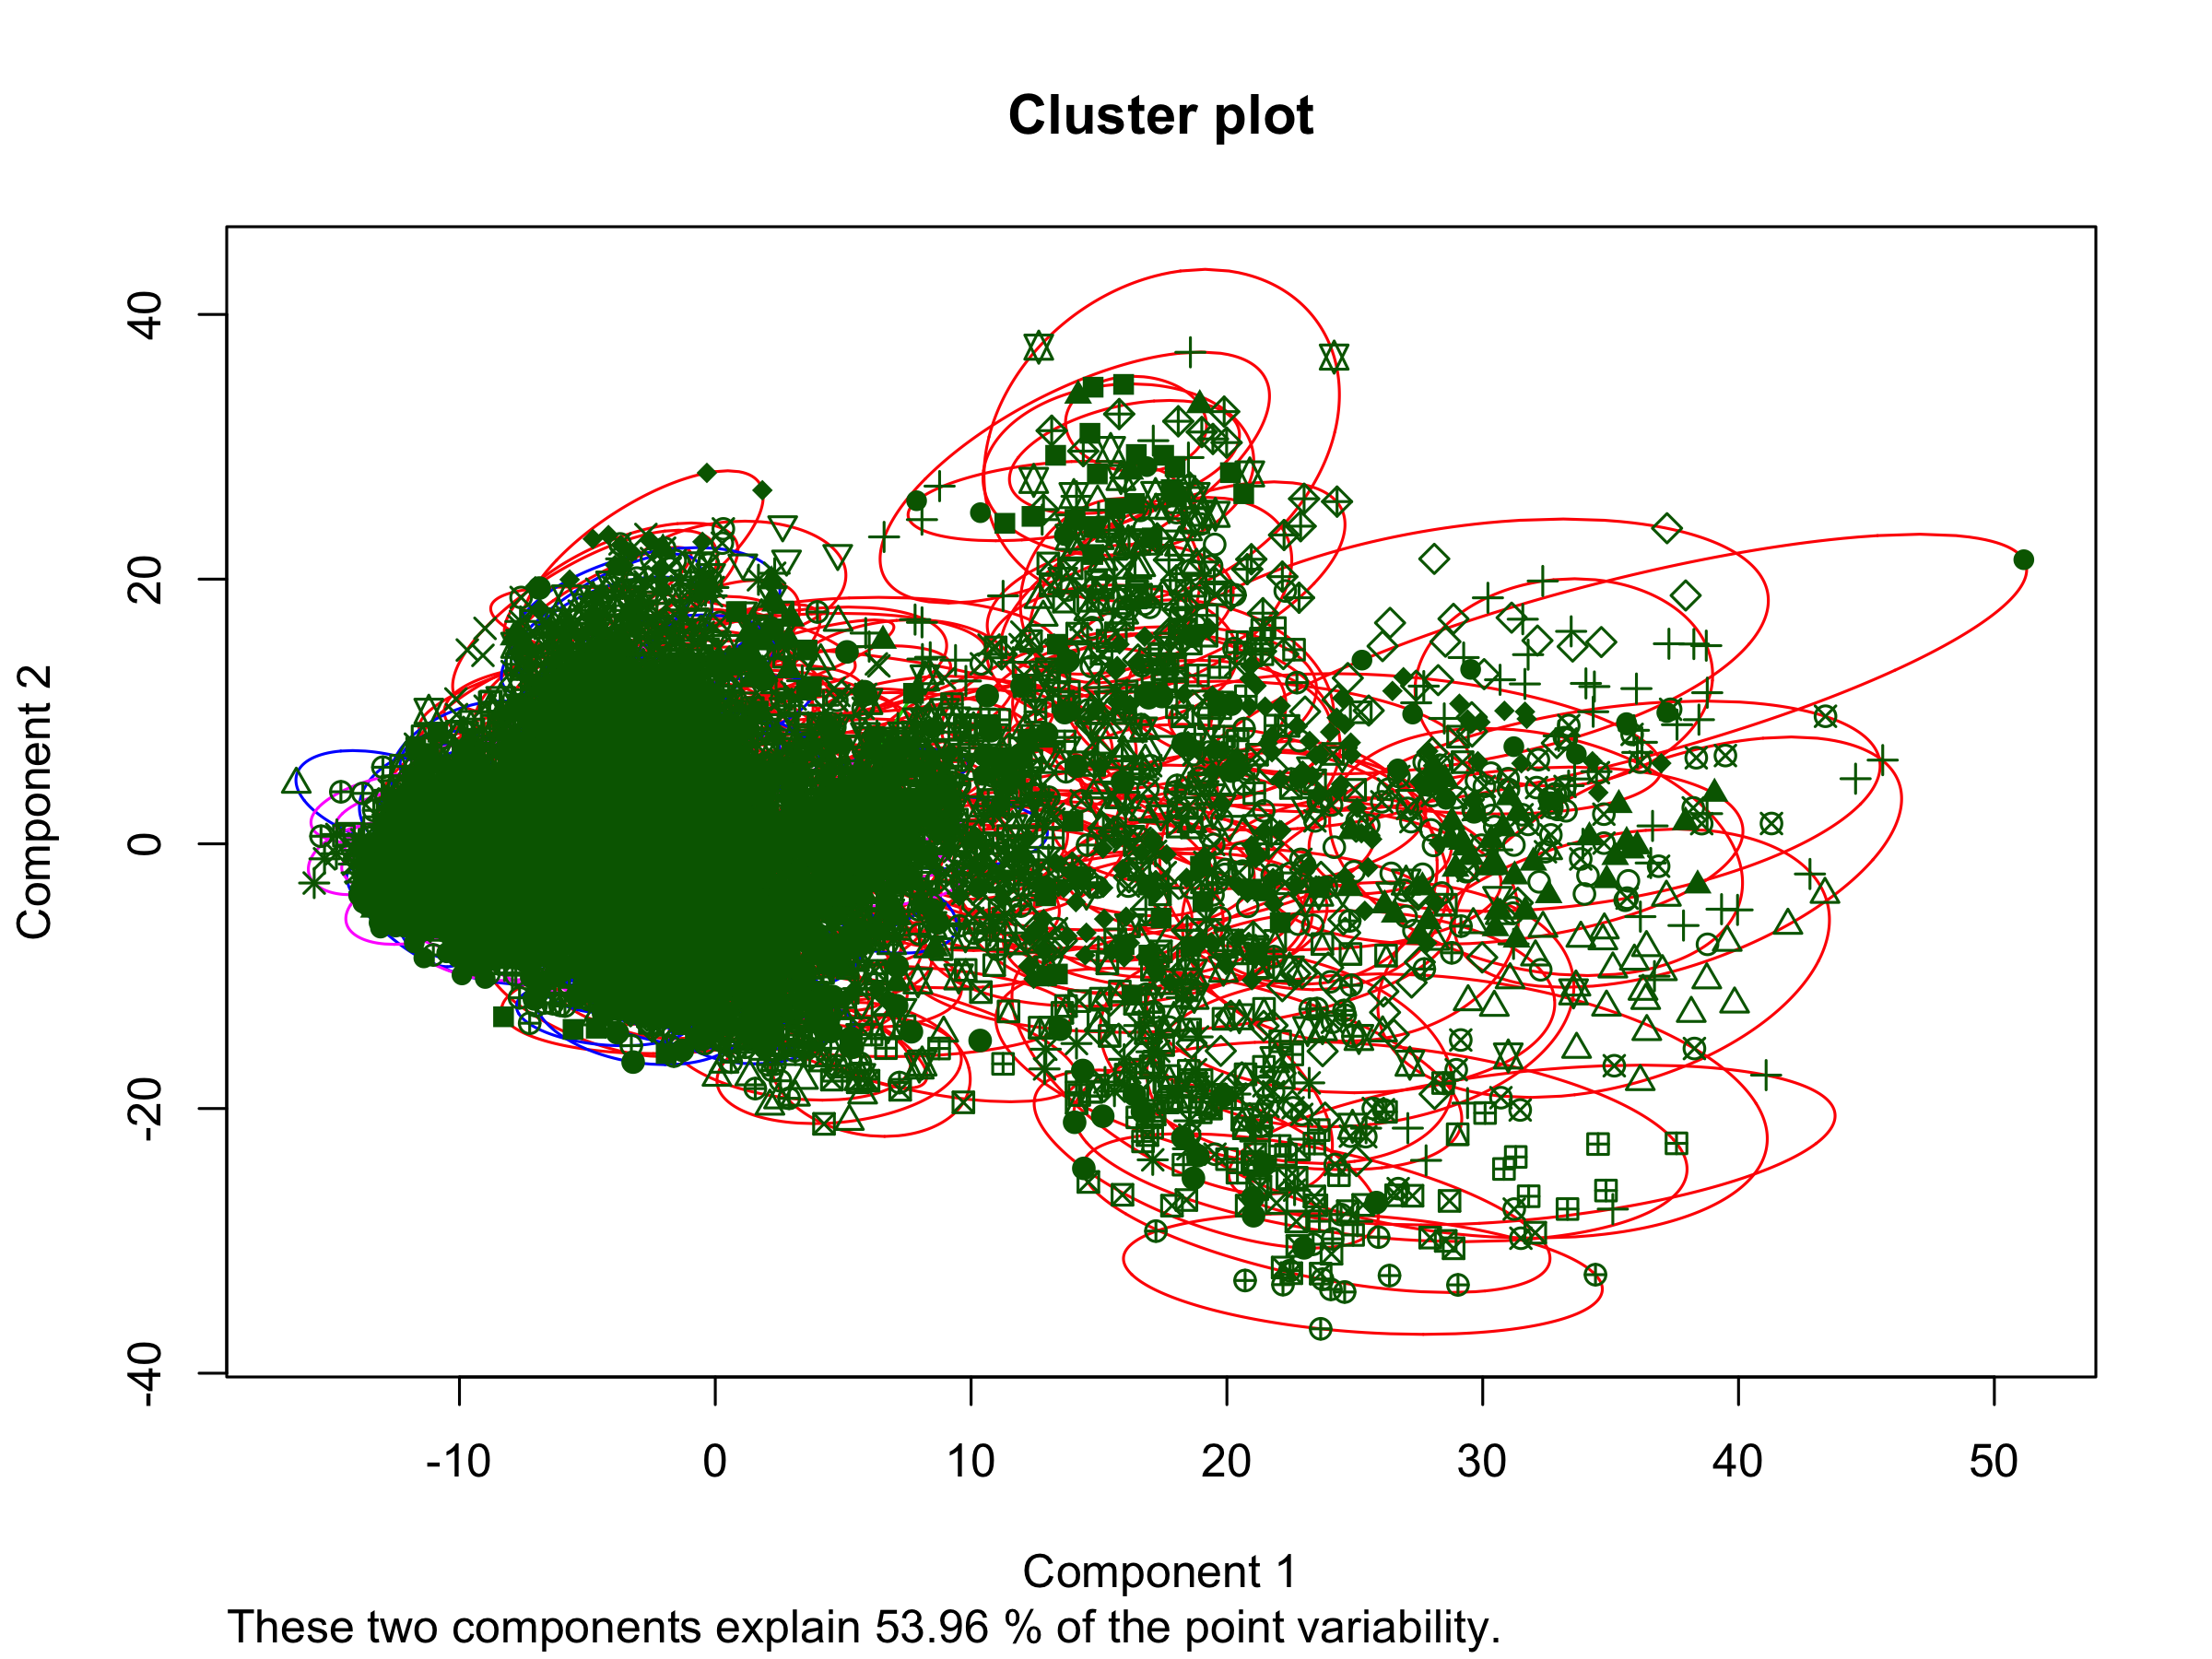
\includegraphics[width = 0.2\textwidth]{clusplot_3.png}\label{fig:3}}\hspace{1em}
%  		
%  		
  		\subfloat[Clustering data consisting of digit 4]{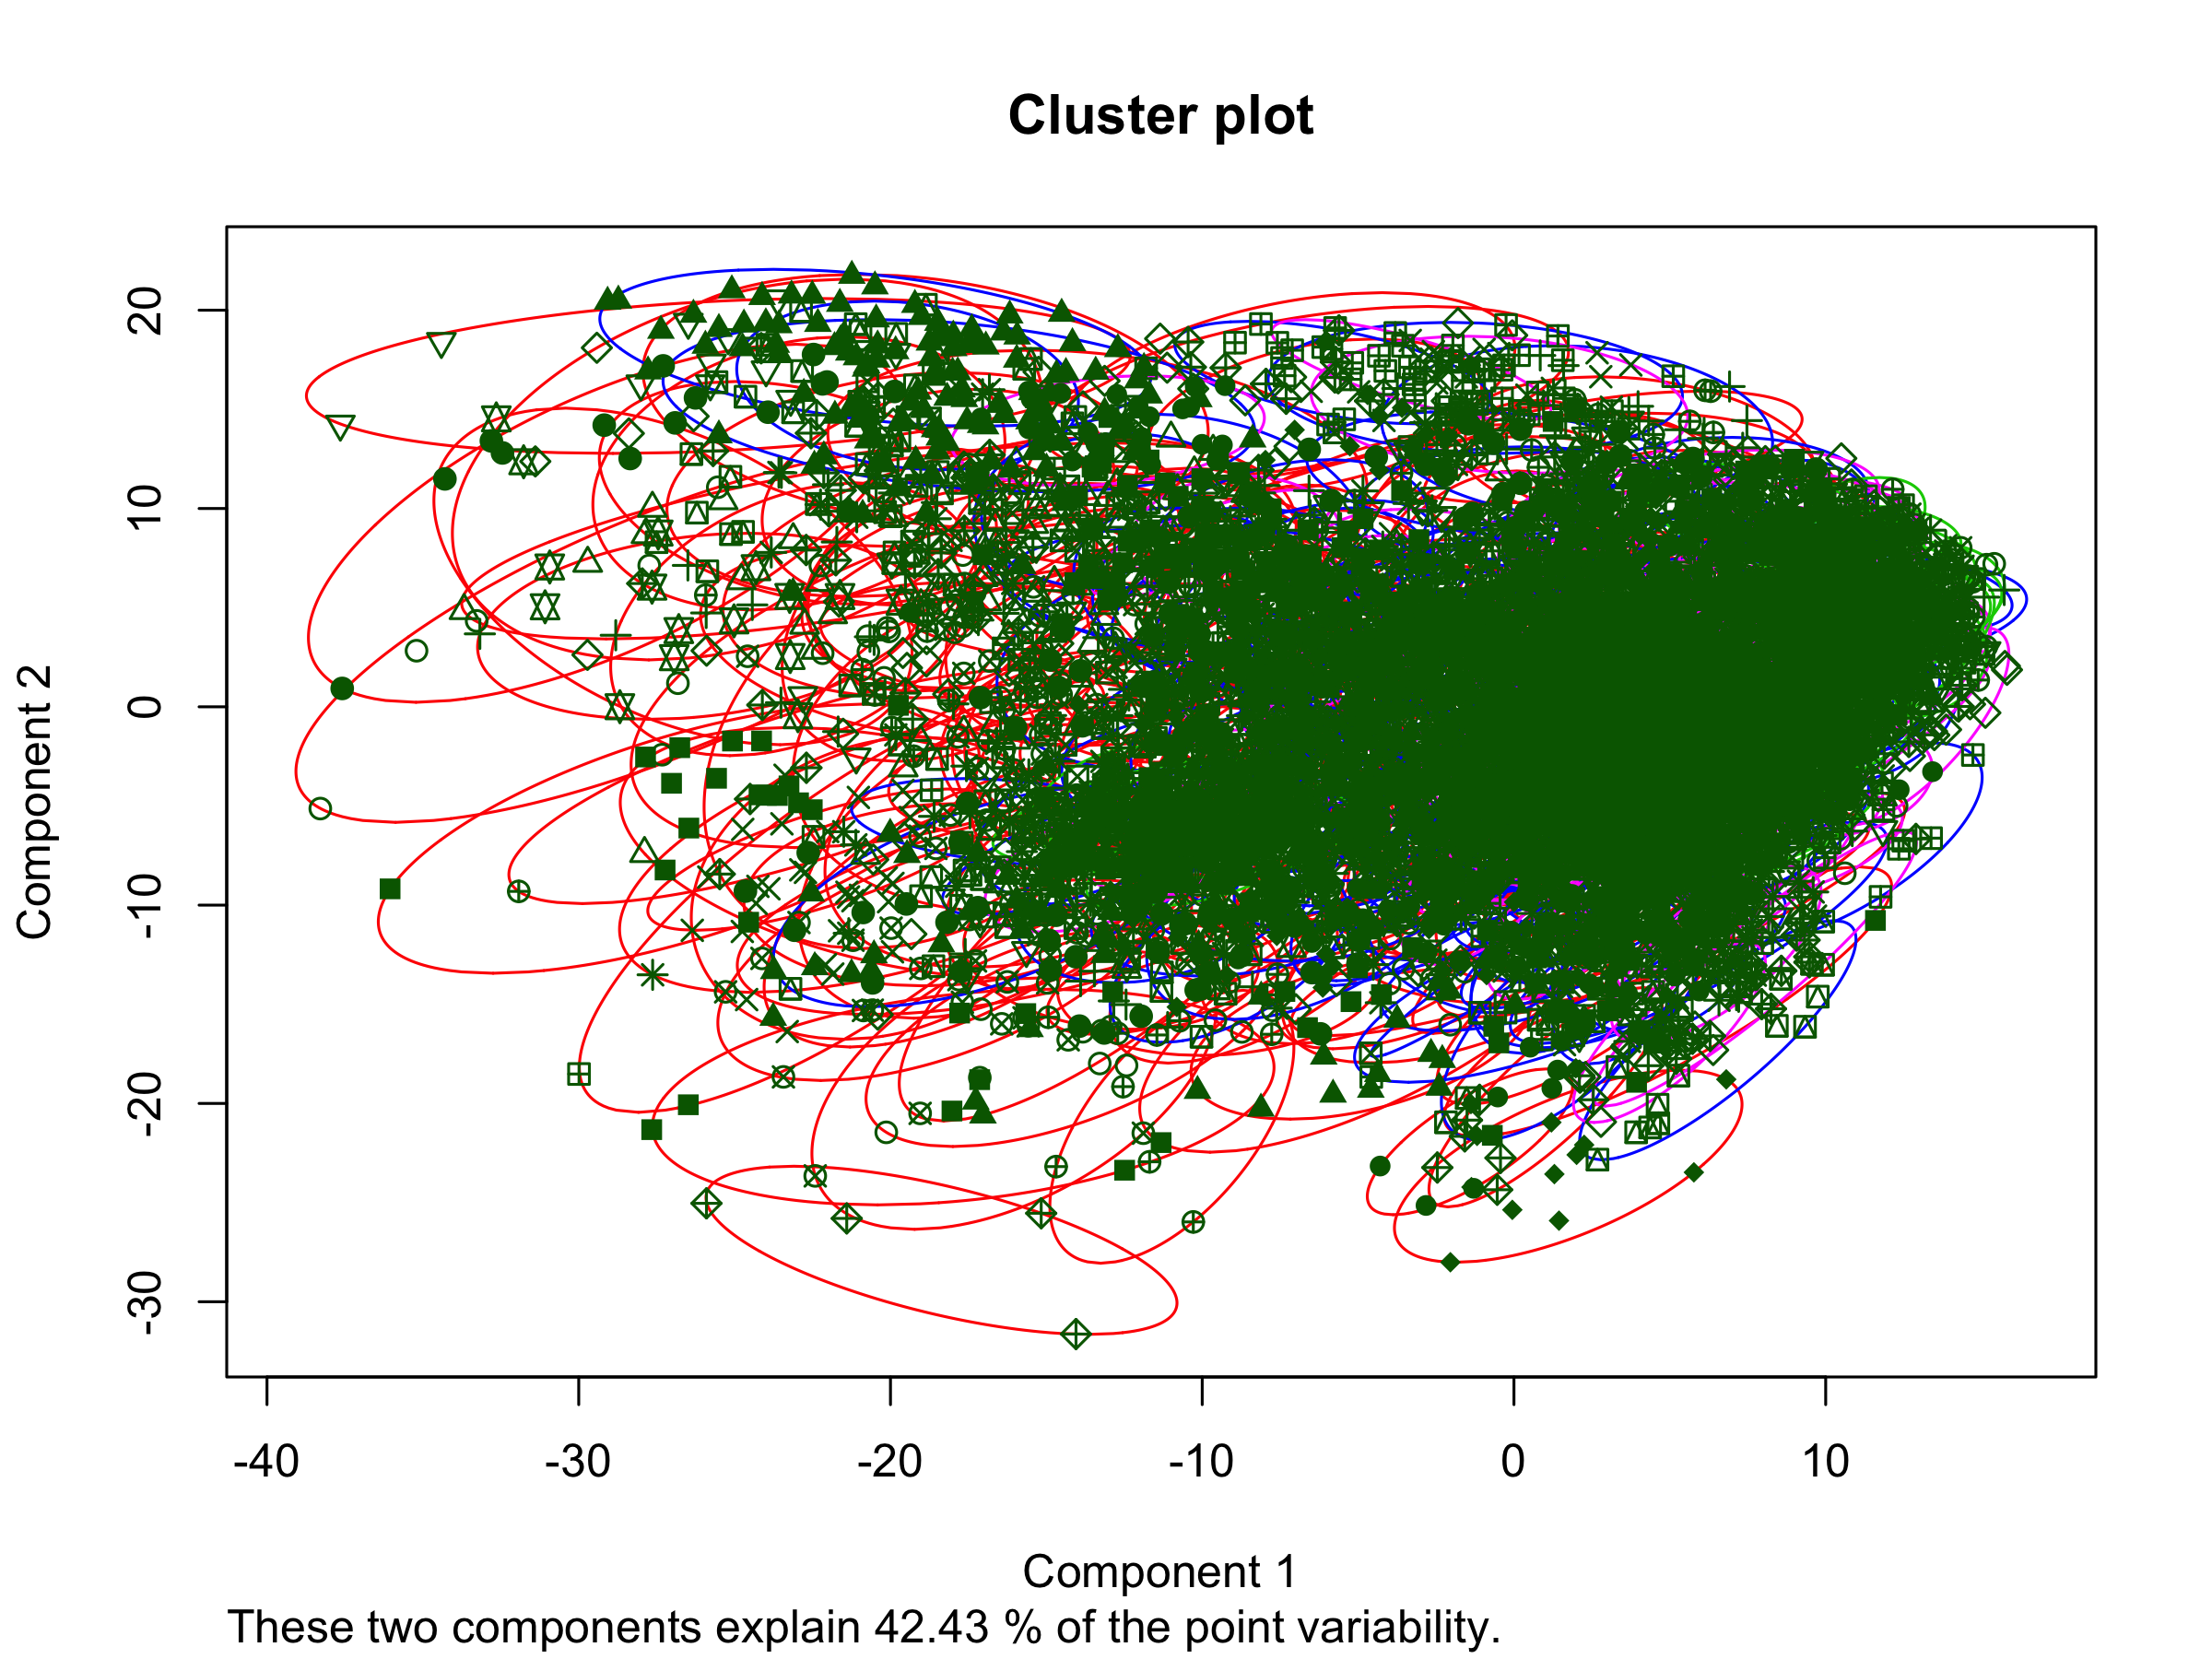
\includegraphics[width = 0.2\textwidth]{clusplot_4.png}\label{fig:4}}
%  		
  		\subfloat[Clustering data consisting of digit 5]{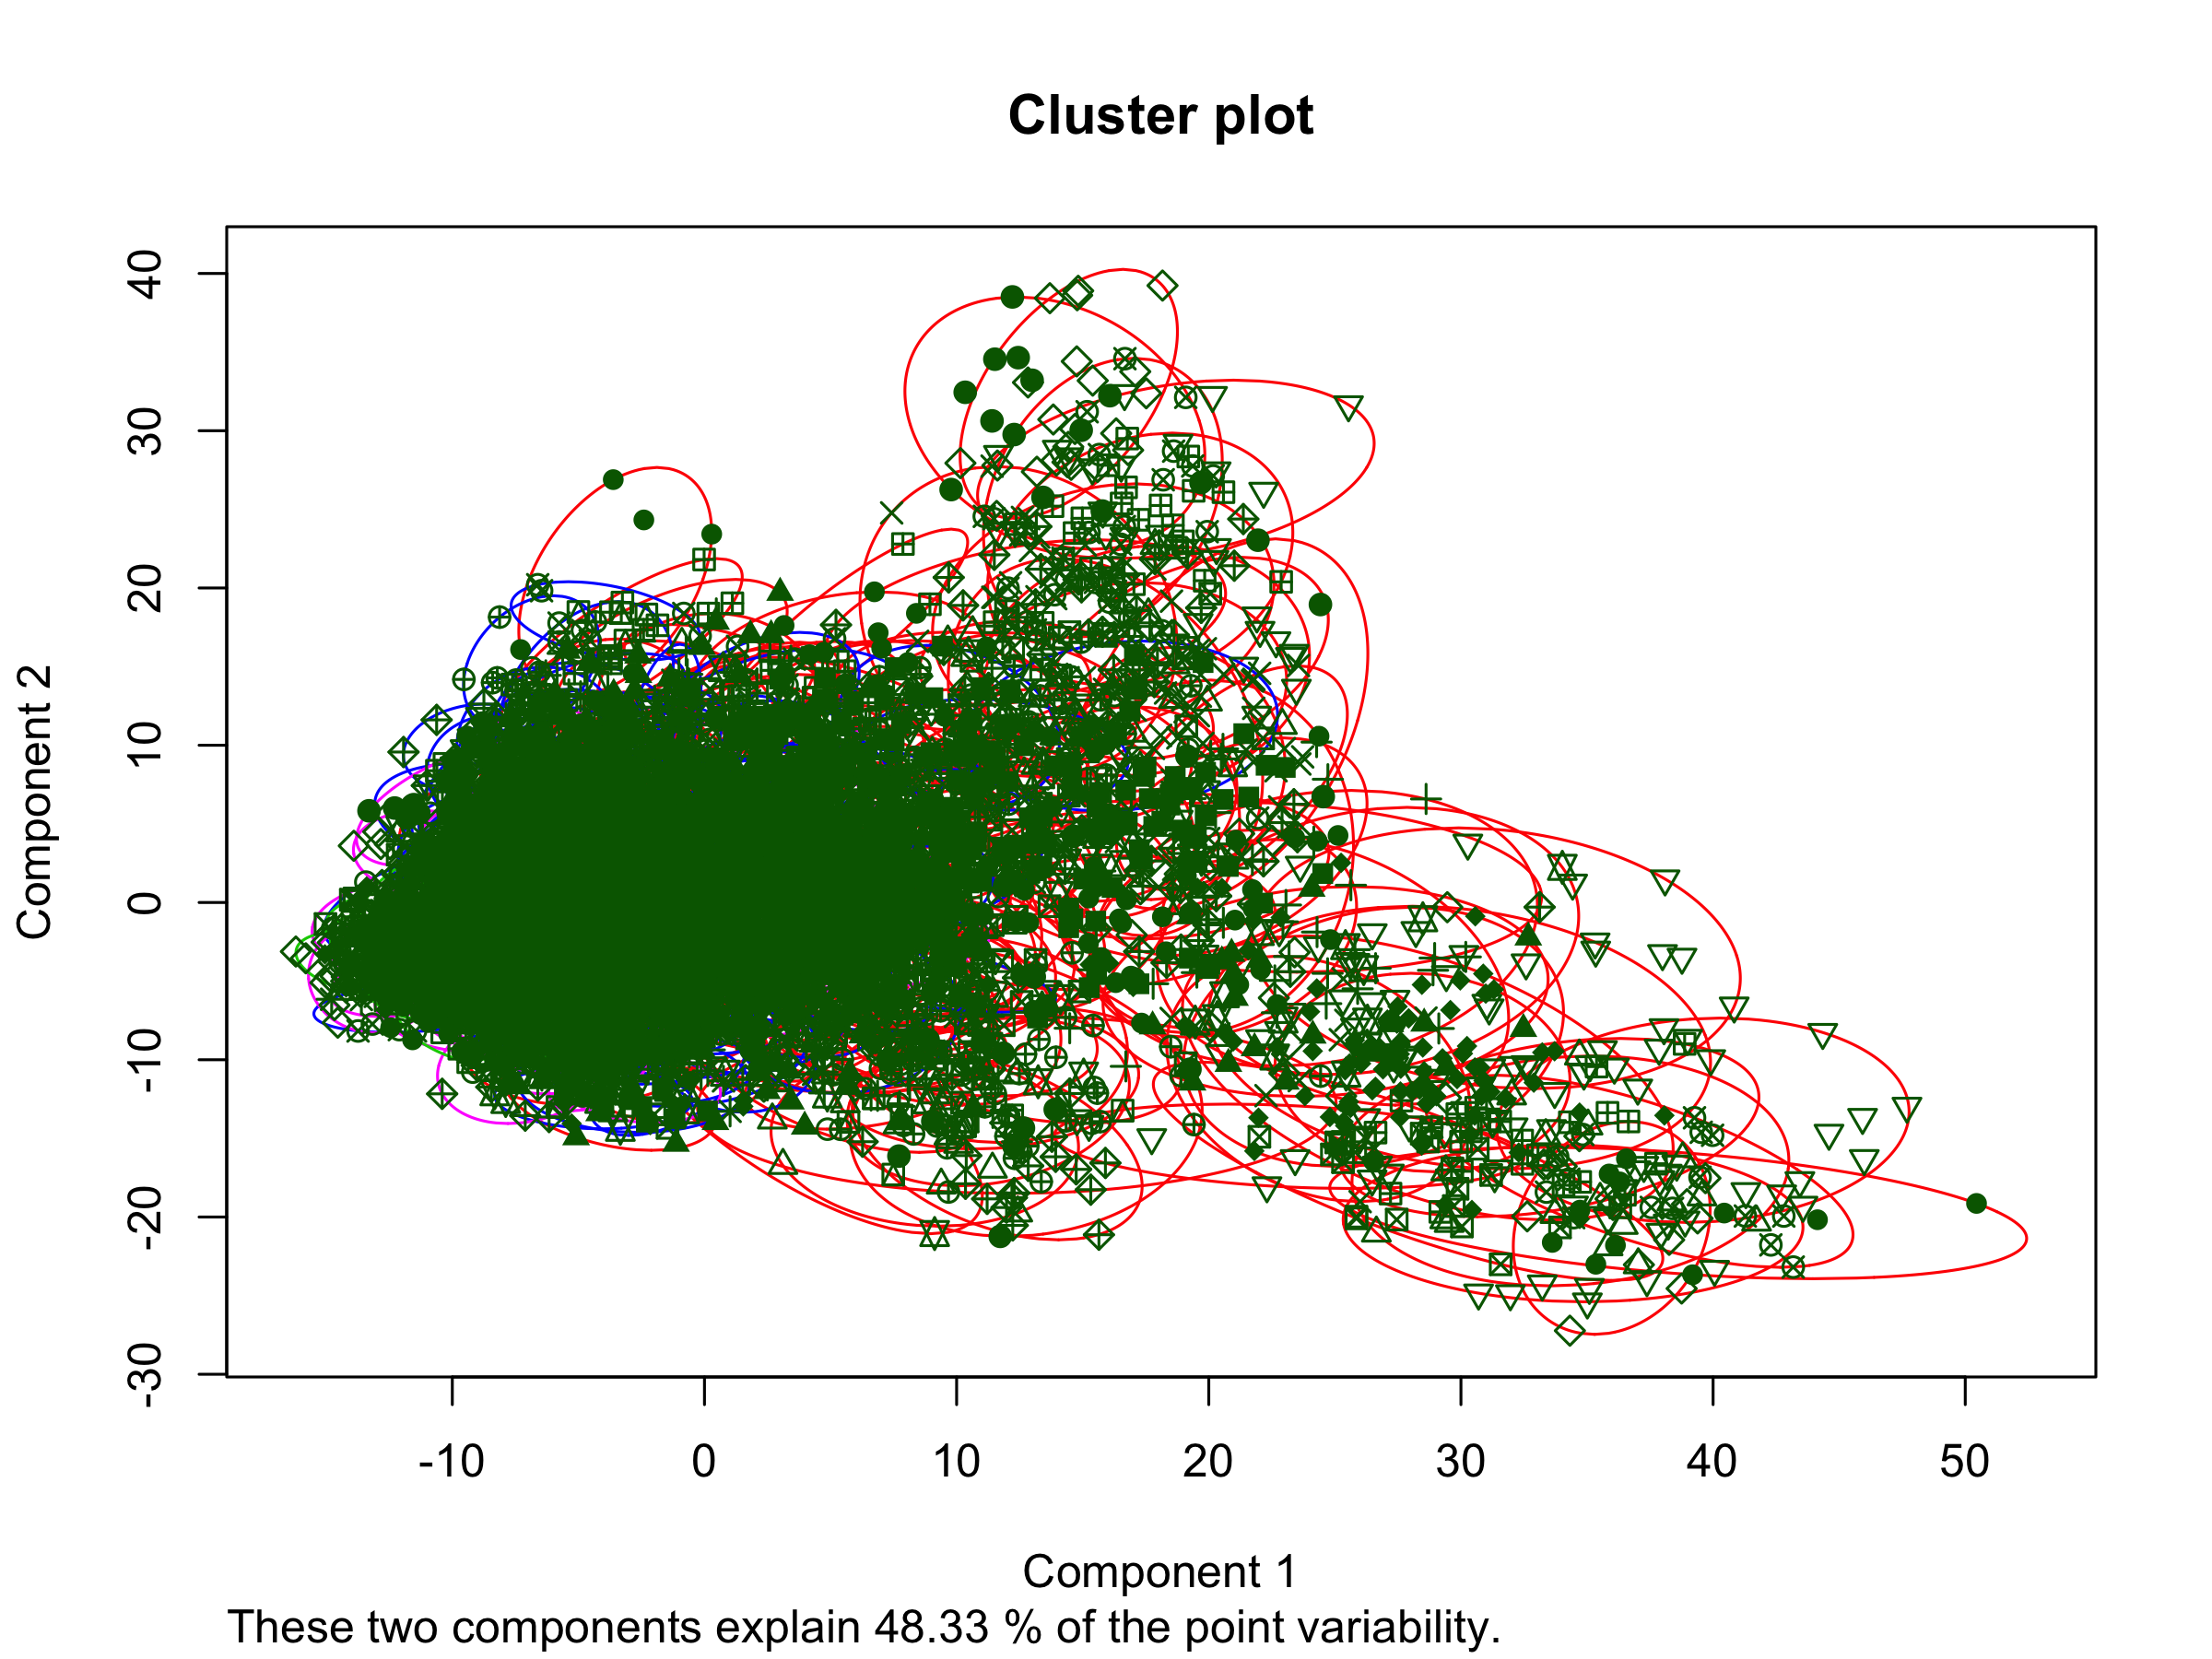
\includegraphics[width = 0.2\textwidth]{clusplot_5.png}\label{fig:5}}
%  			
%  			
 		\subfloat[Clustering data consisting of digit 6]{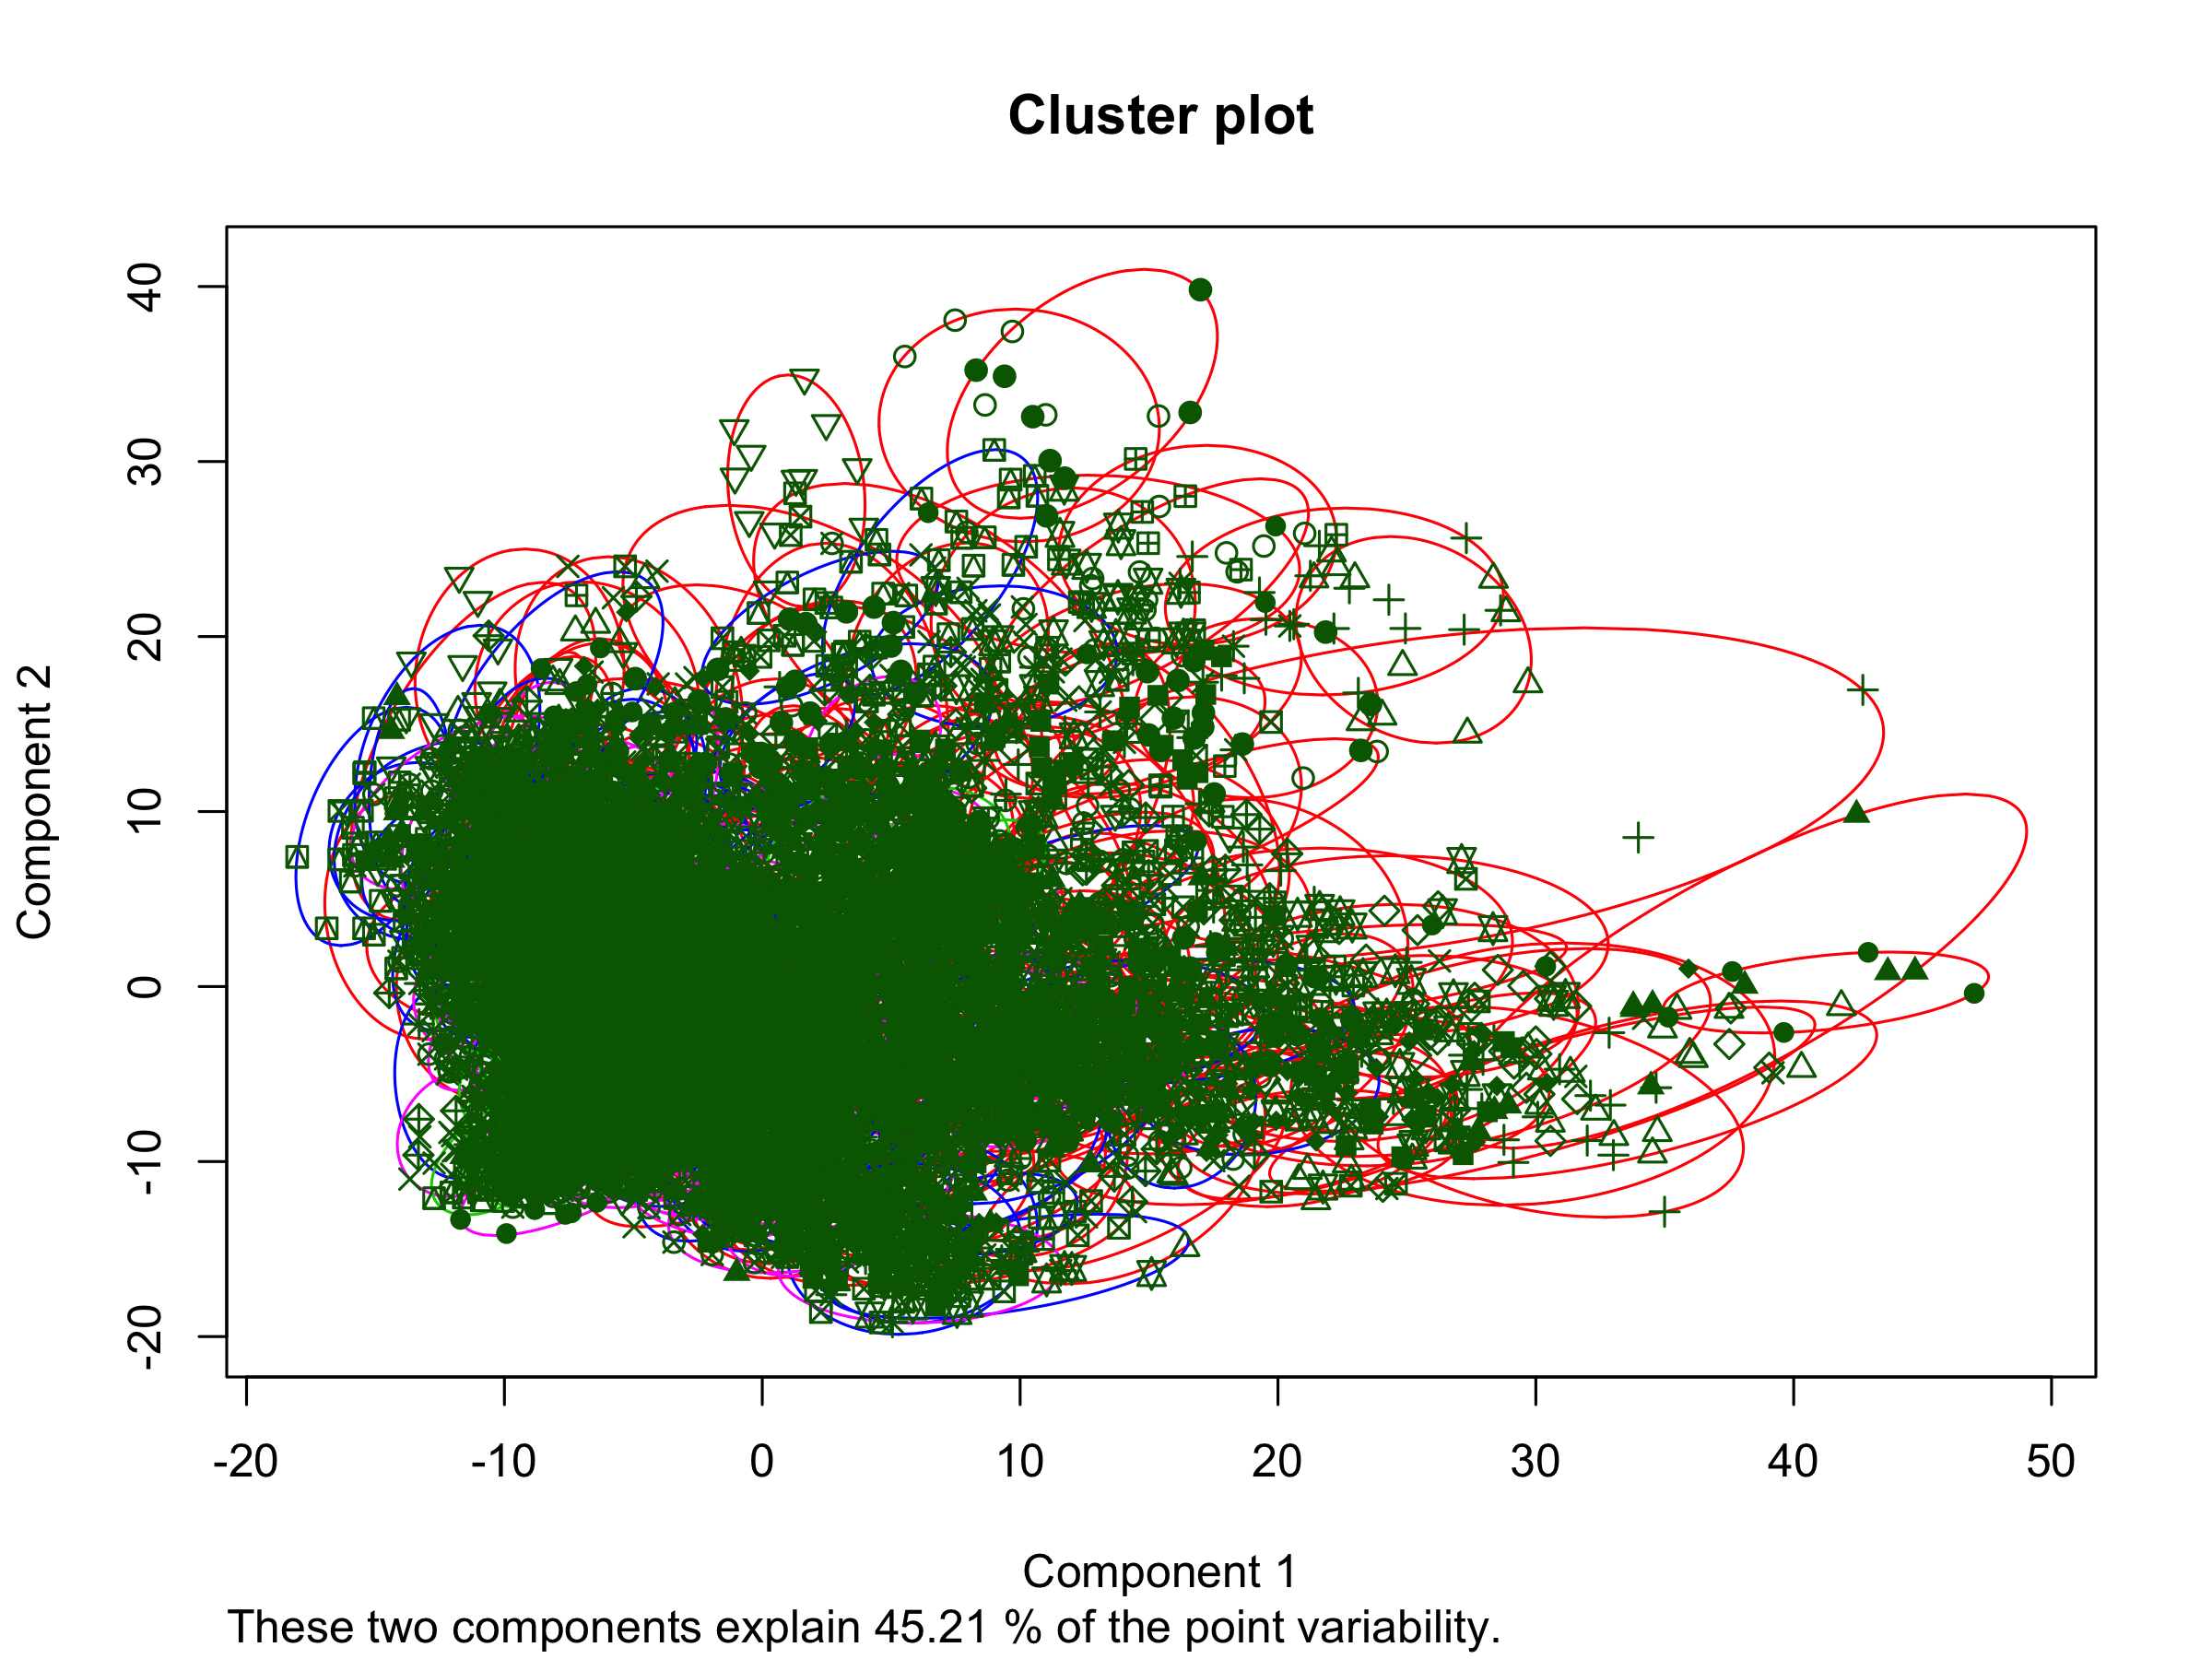
\includegraphics[width = 0.2\textwidth]{clusplot_6.png}\label{fig:6}}\hspace{1em}
%%  		
%%  		
  		\subfloat[Clustering data consisting of digit 7]{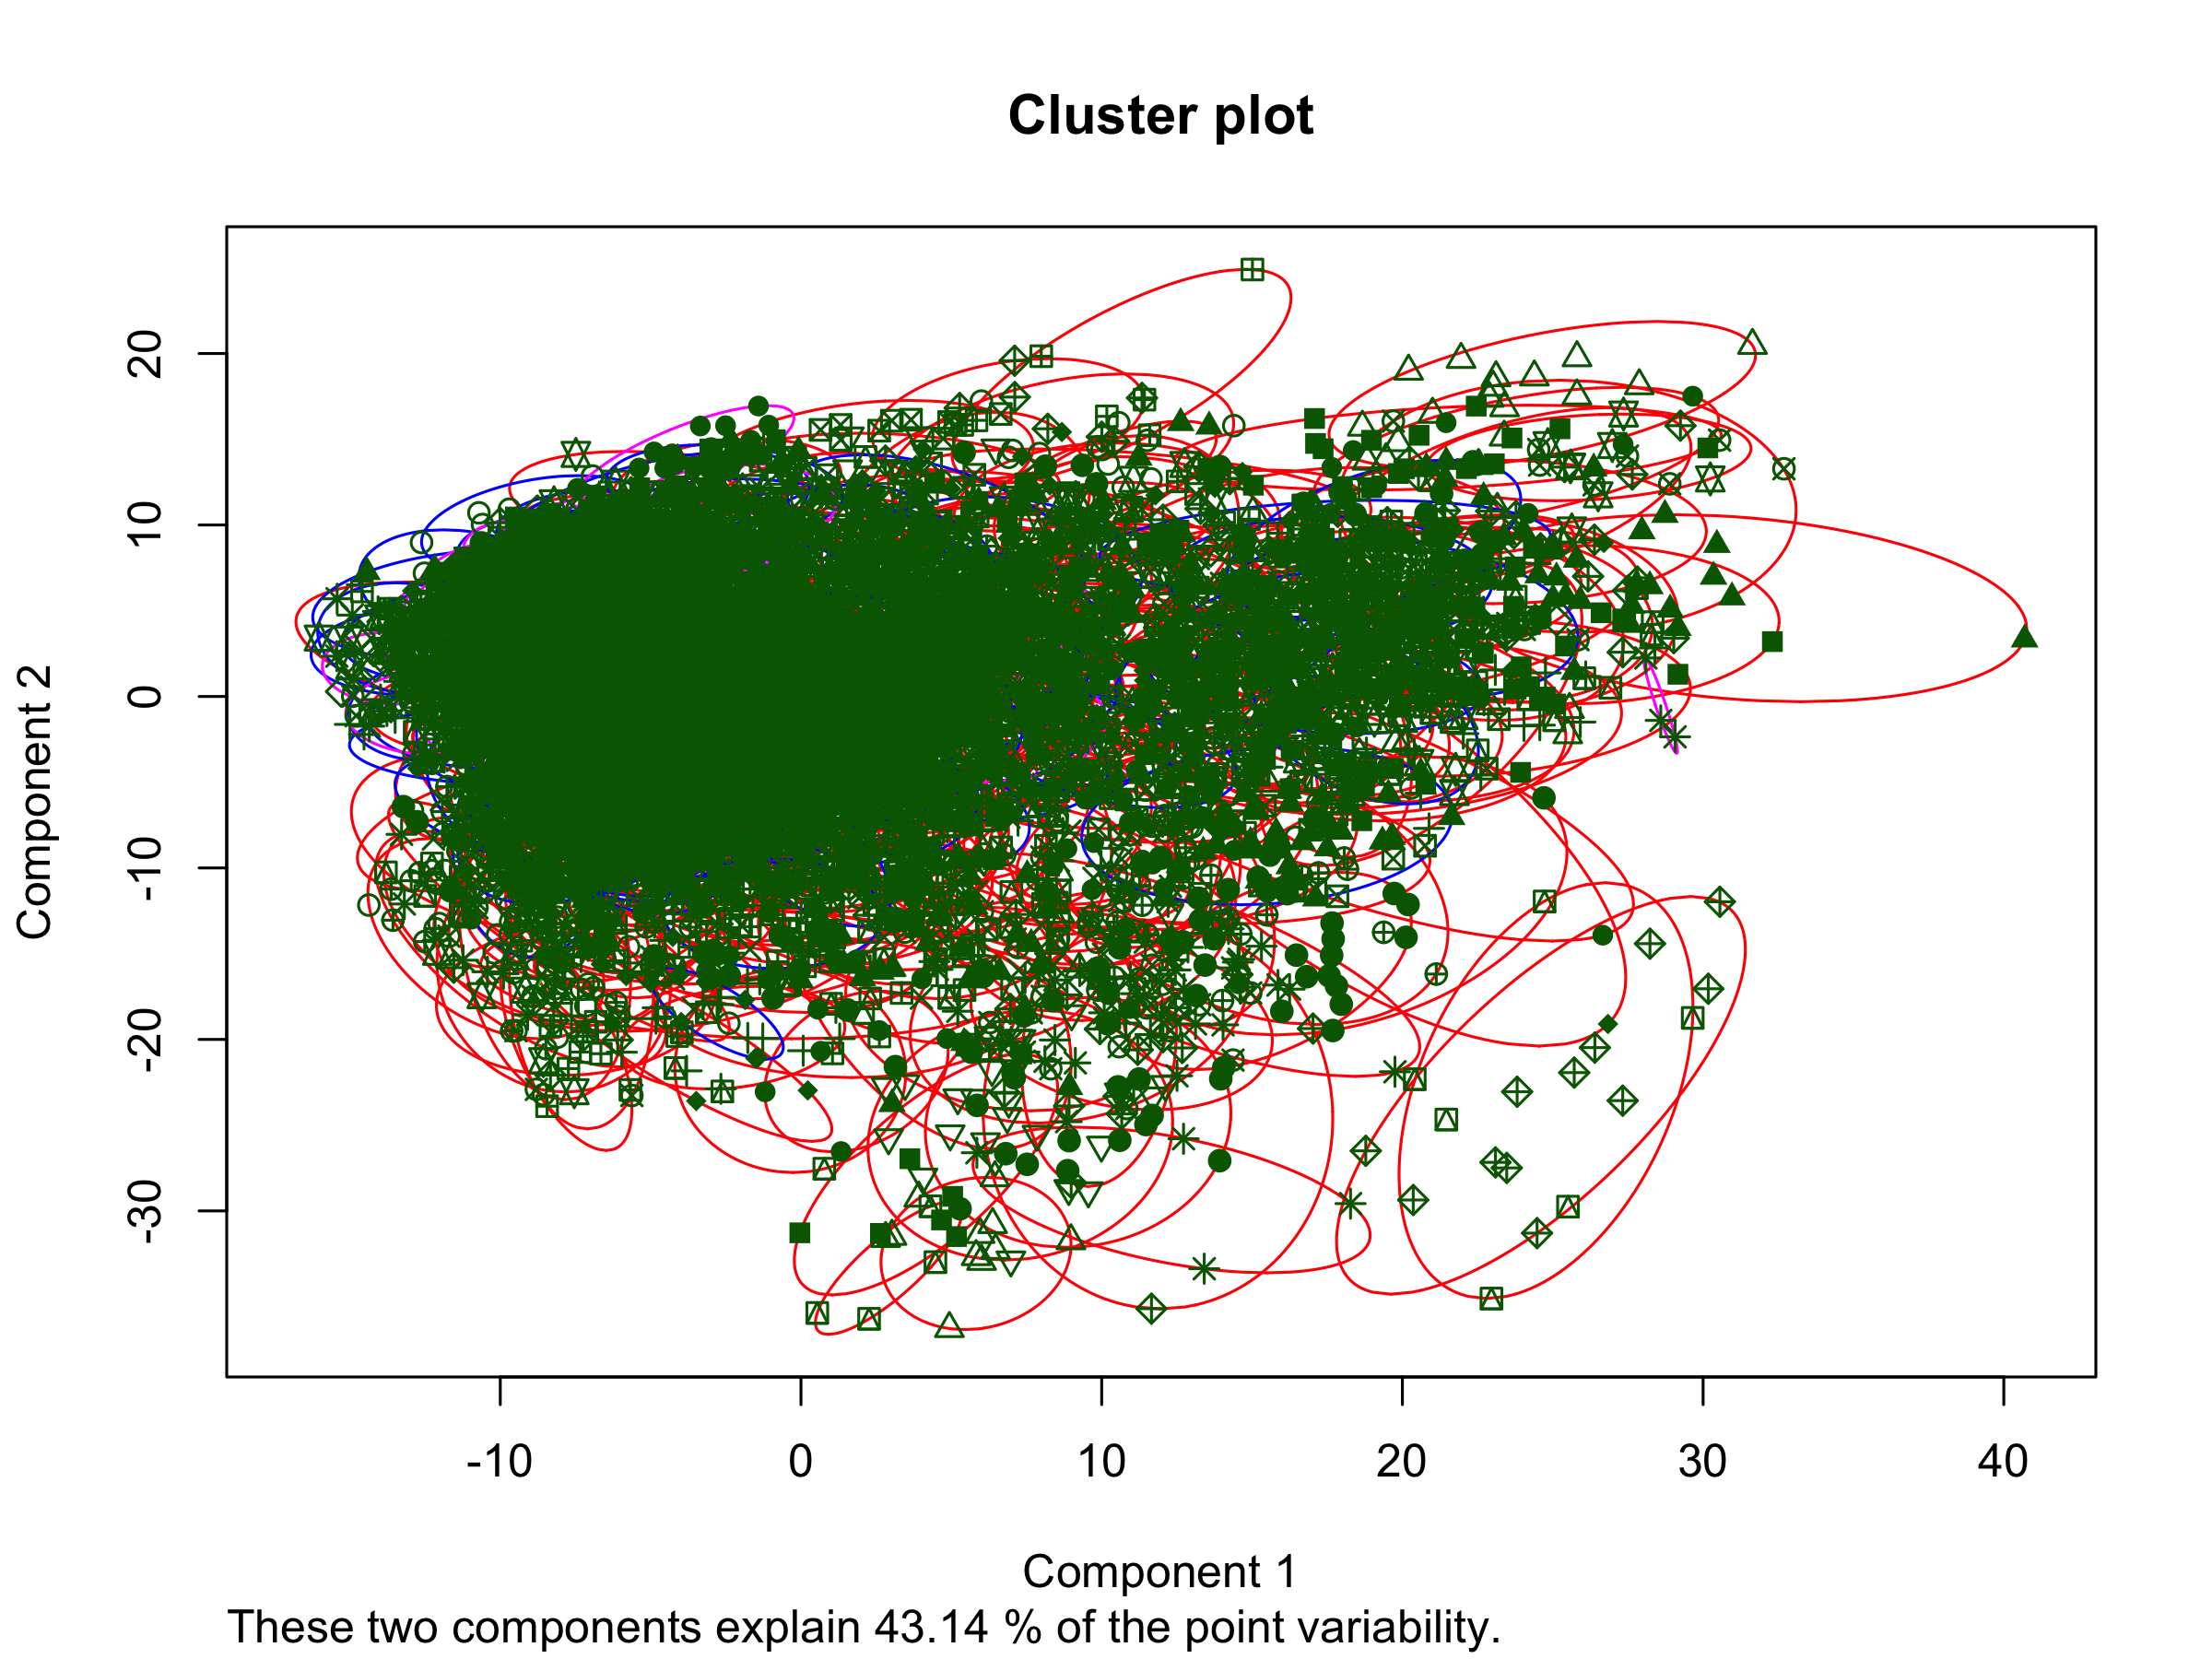
\includegraphics[width = 0.2\textwidth]{clusplot_7.png}\label{fig:7}}
%%
  		\subfloat[Clustering data consisting of digit 8]{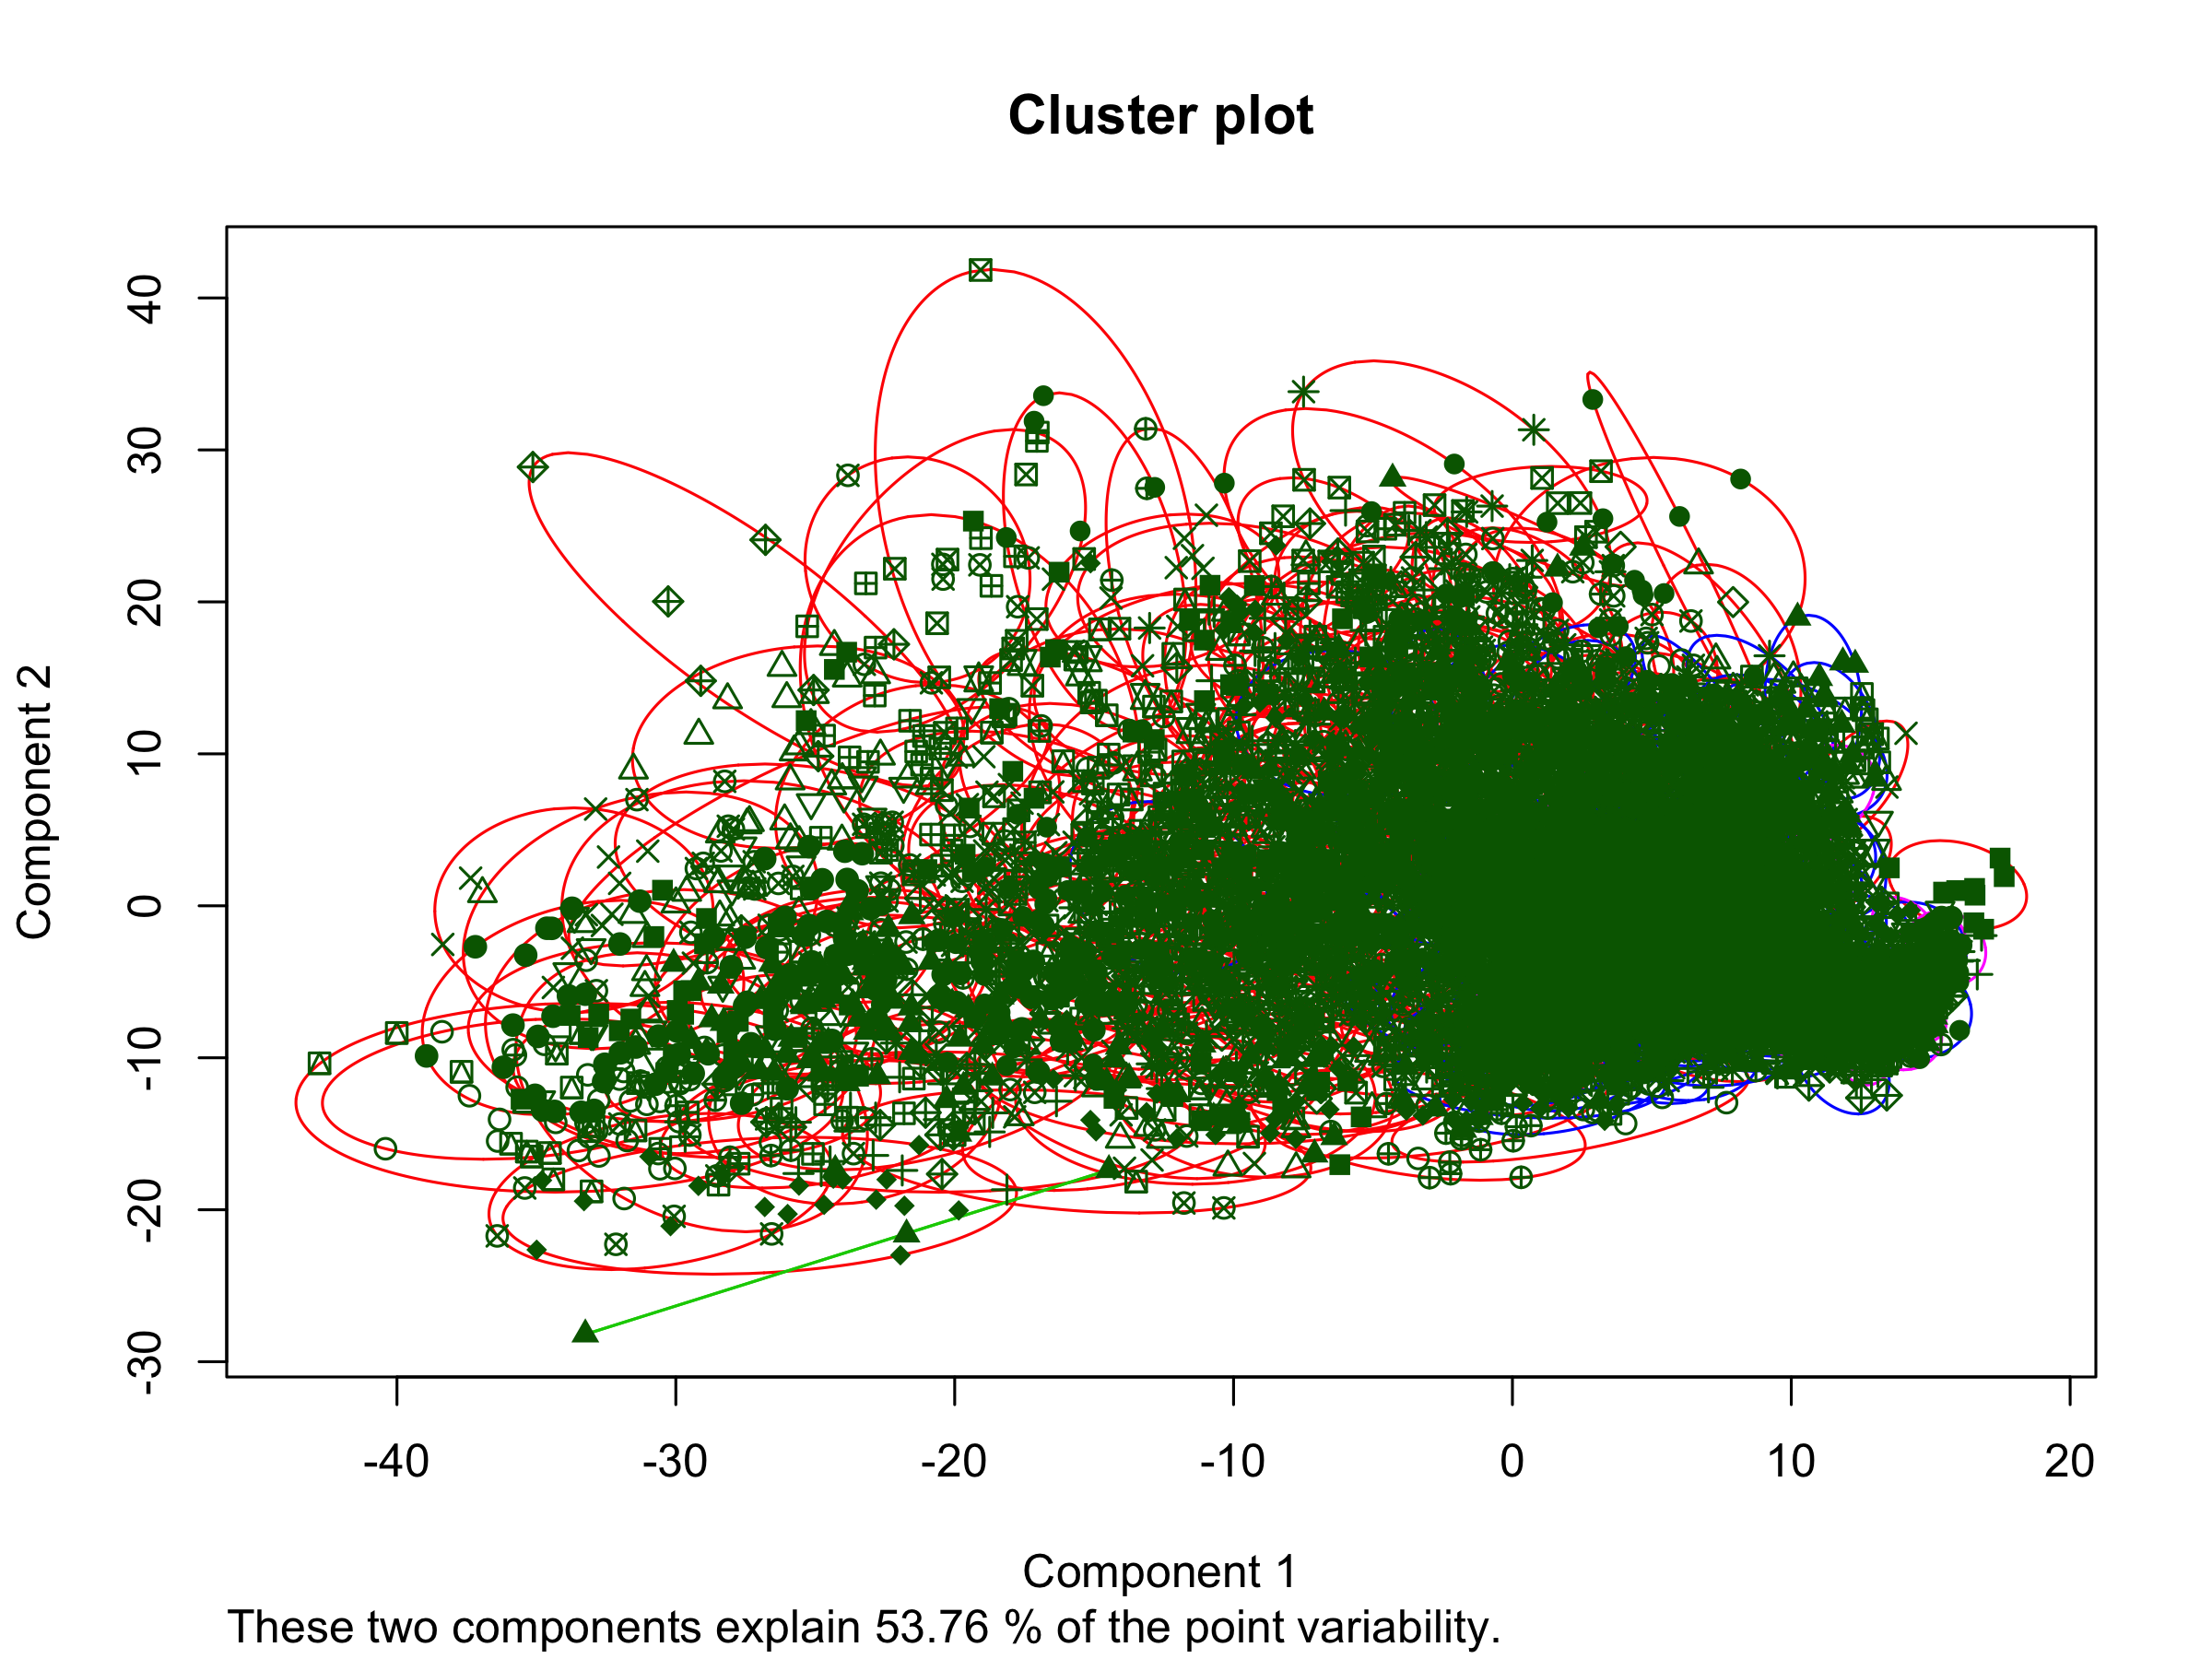
\includegraphics[width = 0.2\textwidth]{clusplot_8.png}\label{fig:8}}
%%  		 
  		 \subfloat[Clustering data consisting of digit 9]{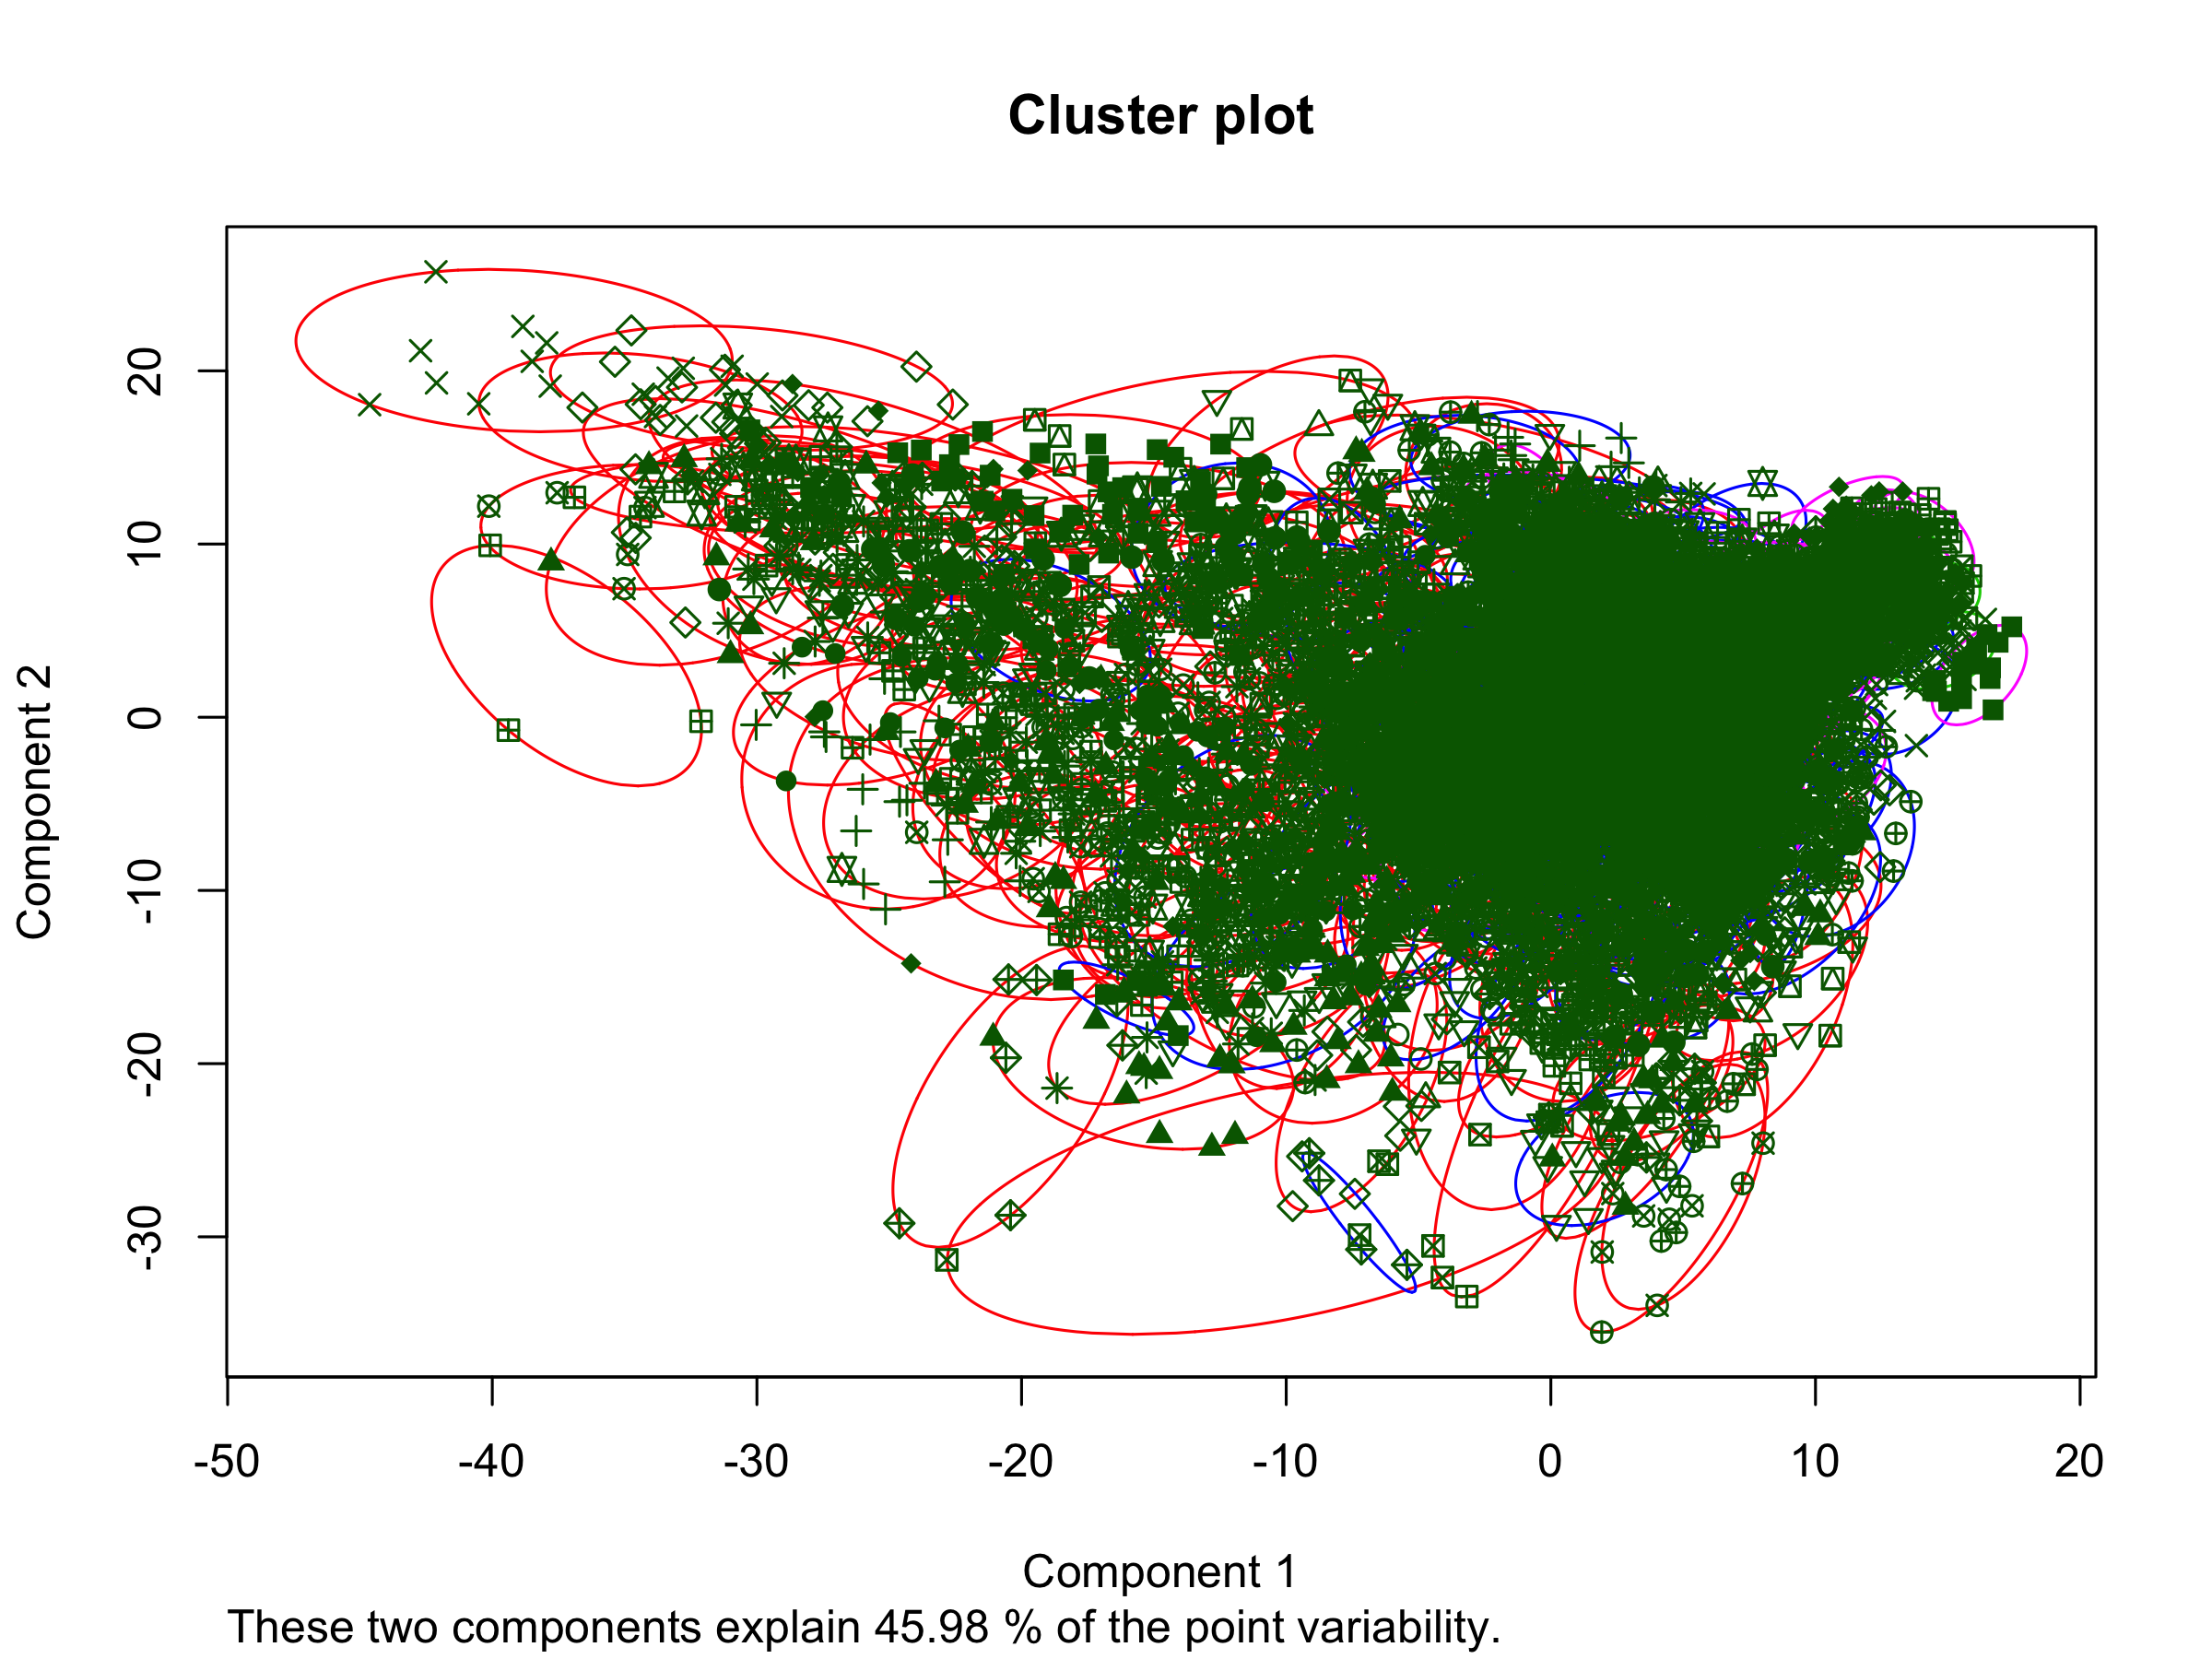
\includegraphics[width = 0.2\textwidth]{clusplot_9.png}\label{fig:9}}\hspace{1em}
\caption{Cluster class distribution and class clustering plots}
\end{figure}


Performing kmeans clustering with 20 cluster took 46 secs, which in general is a huge
improvement compared to kNN. K - means clustering seems more appropriate for big dataset, 
compared to kmeans, purely based on the runtime.   Accuracy wise it seems a bit less accurate,
based the amount information is shared amoung each cluster. 
When using kNN was very in unlikely that an digit would be misclassified based on the
confusionmatrix  in figure \ref{fig:confusionMatrixAll}, but using kmeans doesn't classify as
accurate as knn which can be seen in \ref{fig:complete} where a lot of different classes overlap
different clusters making it hard to distinctly say whether an test data belongs to
one certain class. 

The dendrogram of figure \ref{fig:dendo} visualizes
the digit class clustering, where eg. "X1" represents the digit 1.
Asides from a within-digit similarity, this dendrogram also
hints at a similarity between digits 5 and 6, which,
perhaps, is not surprising as these digits often look similar.

Compared to the confusion matrix of figure \ref{fig:confusionMatrixAll},
the dendrogram quickly groups together a 2 and a 7,
which are among the most often confused digits.
Perhaps this is an indication that too aggressive clustering
will group together examples of different digits
early on, which is an undesired effect of clustering;
It means the number of clusters has to be relatively high
to withstand the similarities between examples of different digits.

\begin{figure}[H]
\centering
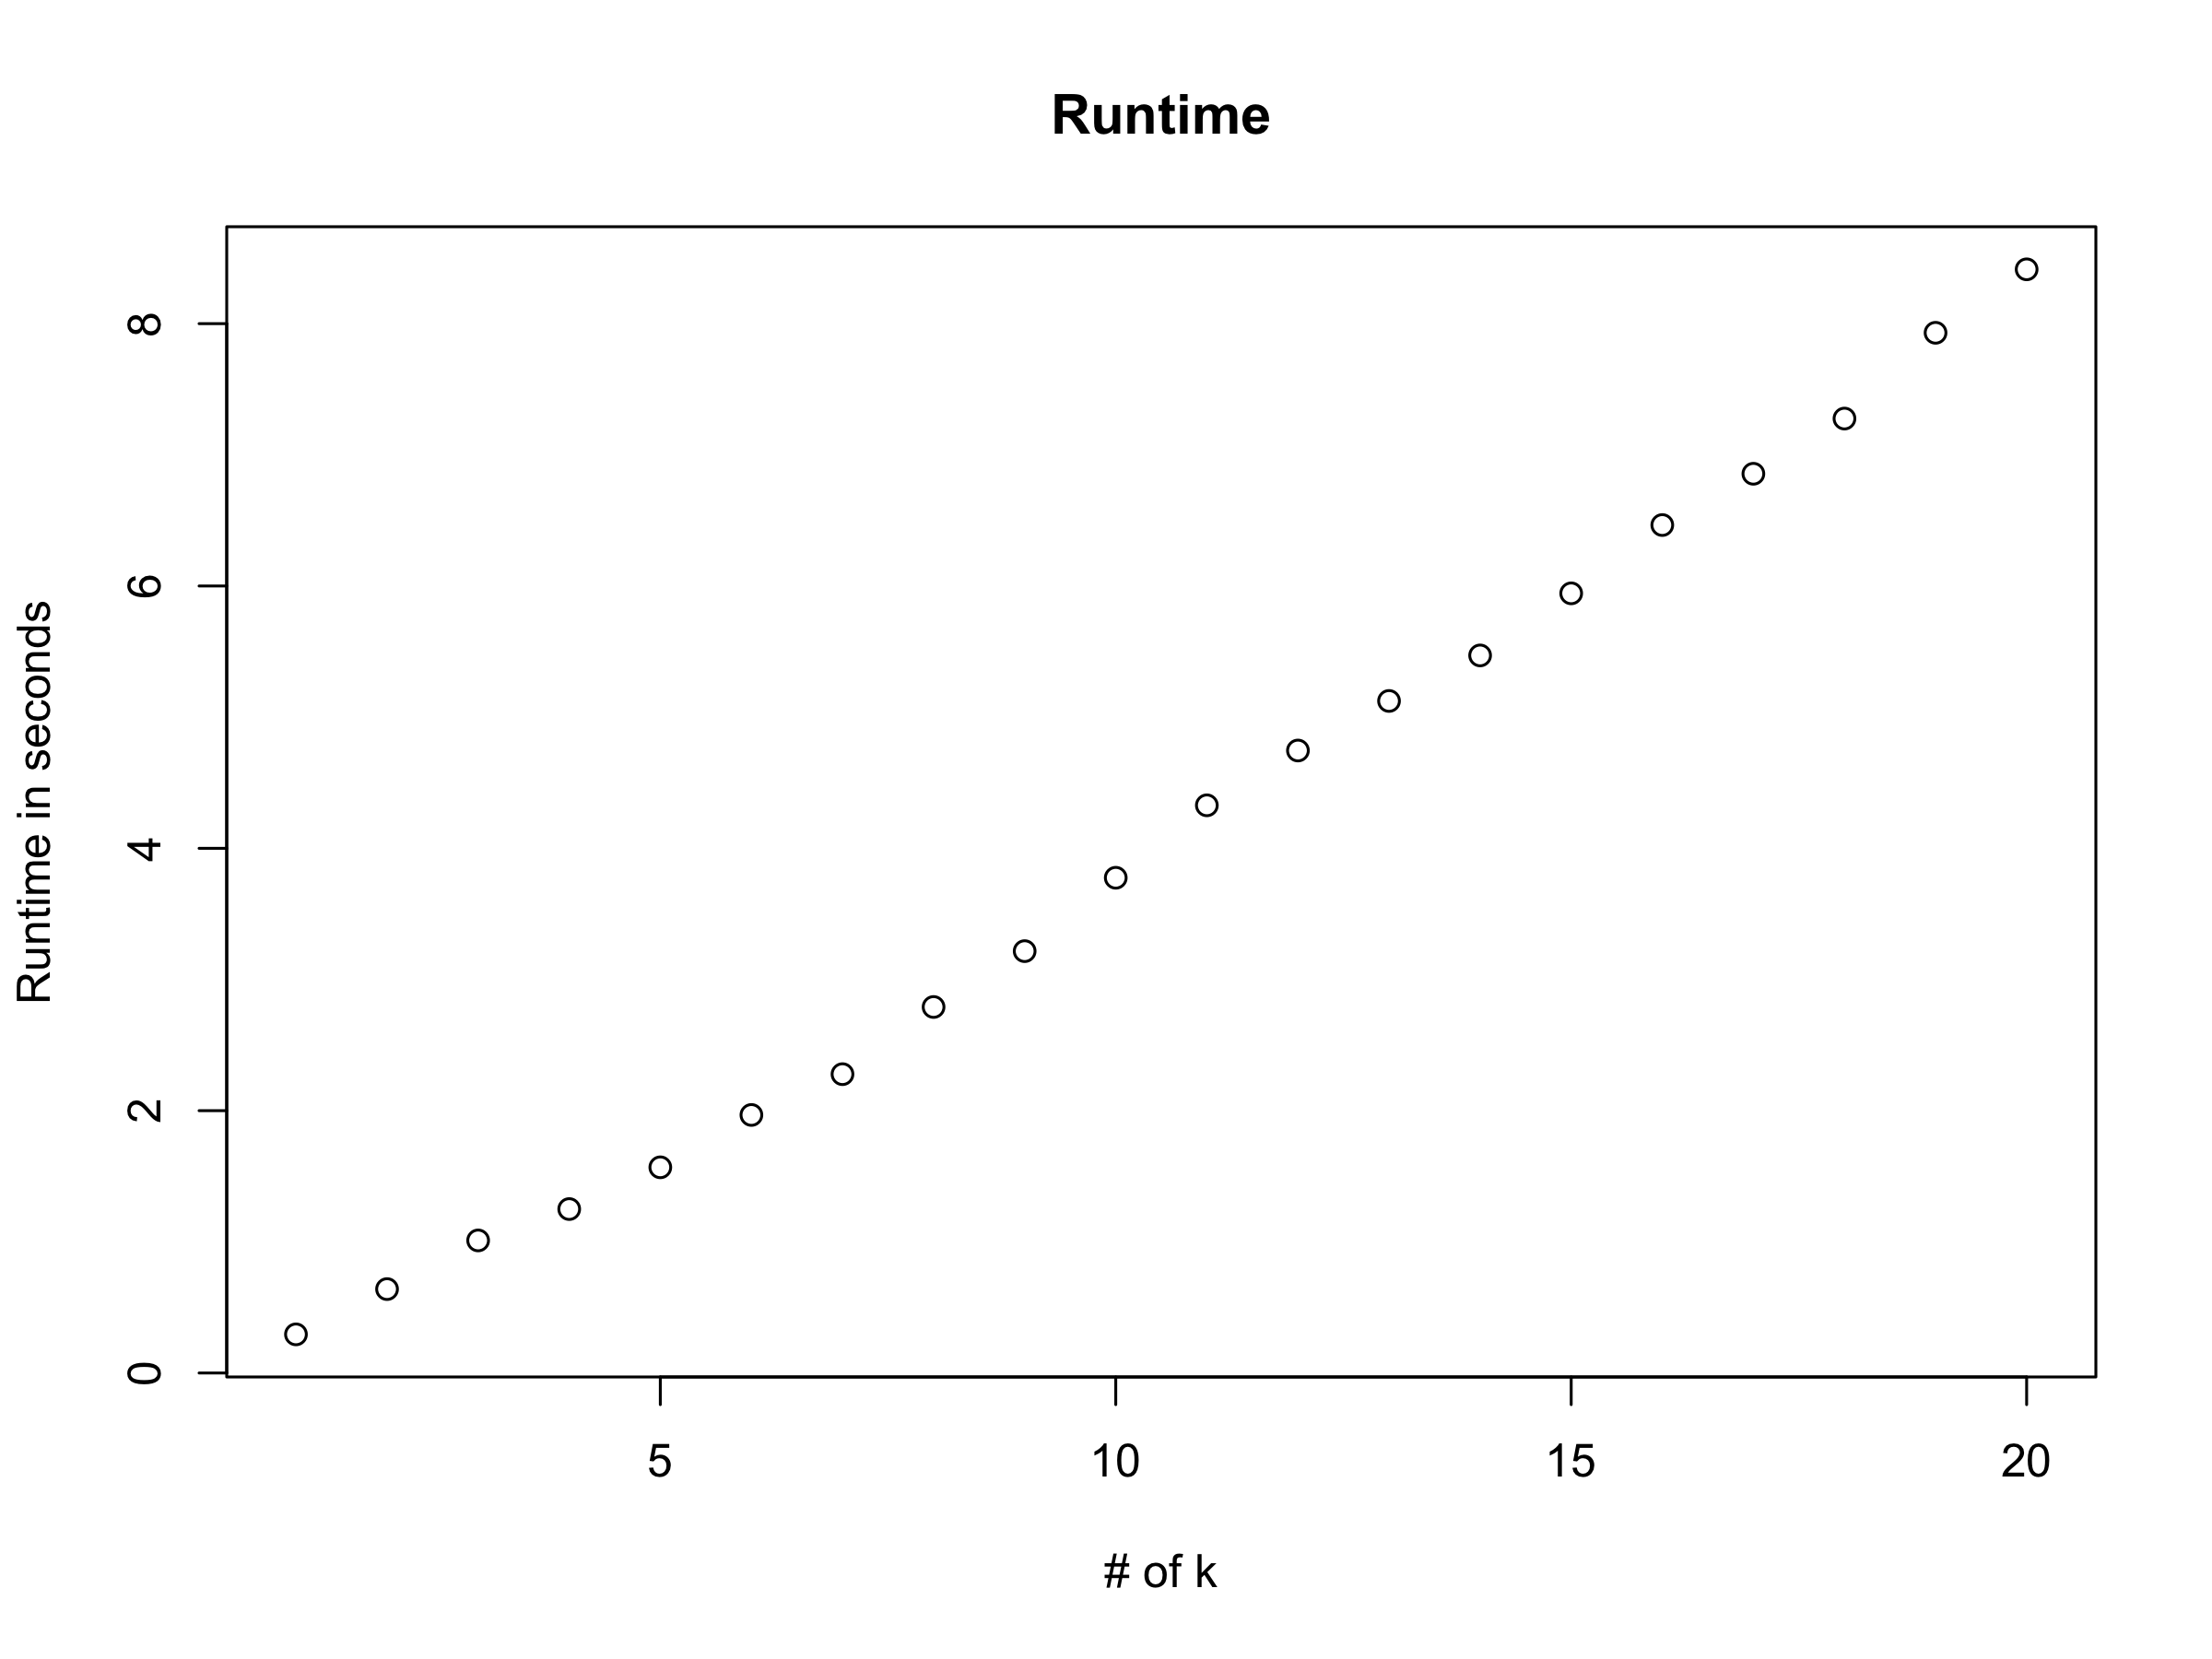
\includegraphics[width = 0.7\textwidth]{runtime.png}
\caption{Runtime of k-means clustering for 20 clusters}
\label{fig:runtime}
\end{figure}

\begin{figure}[H]
		\centering
		 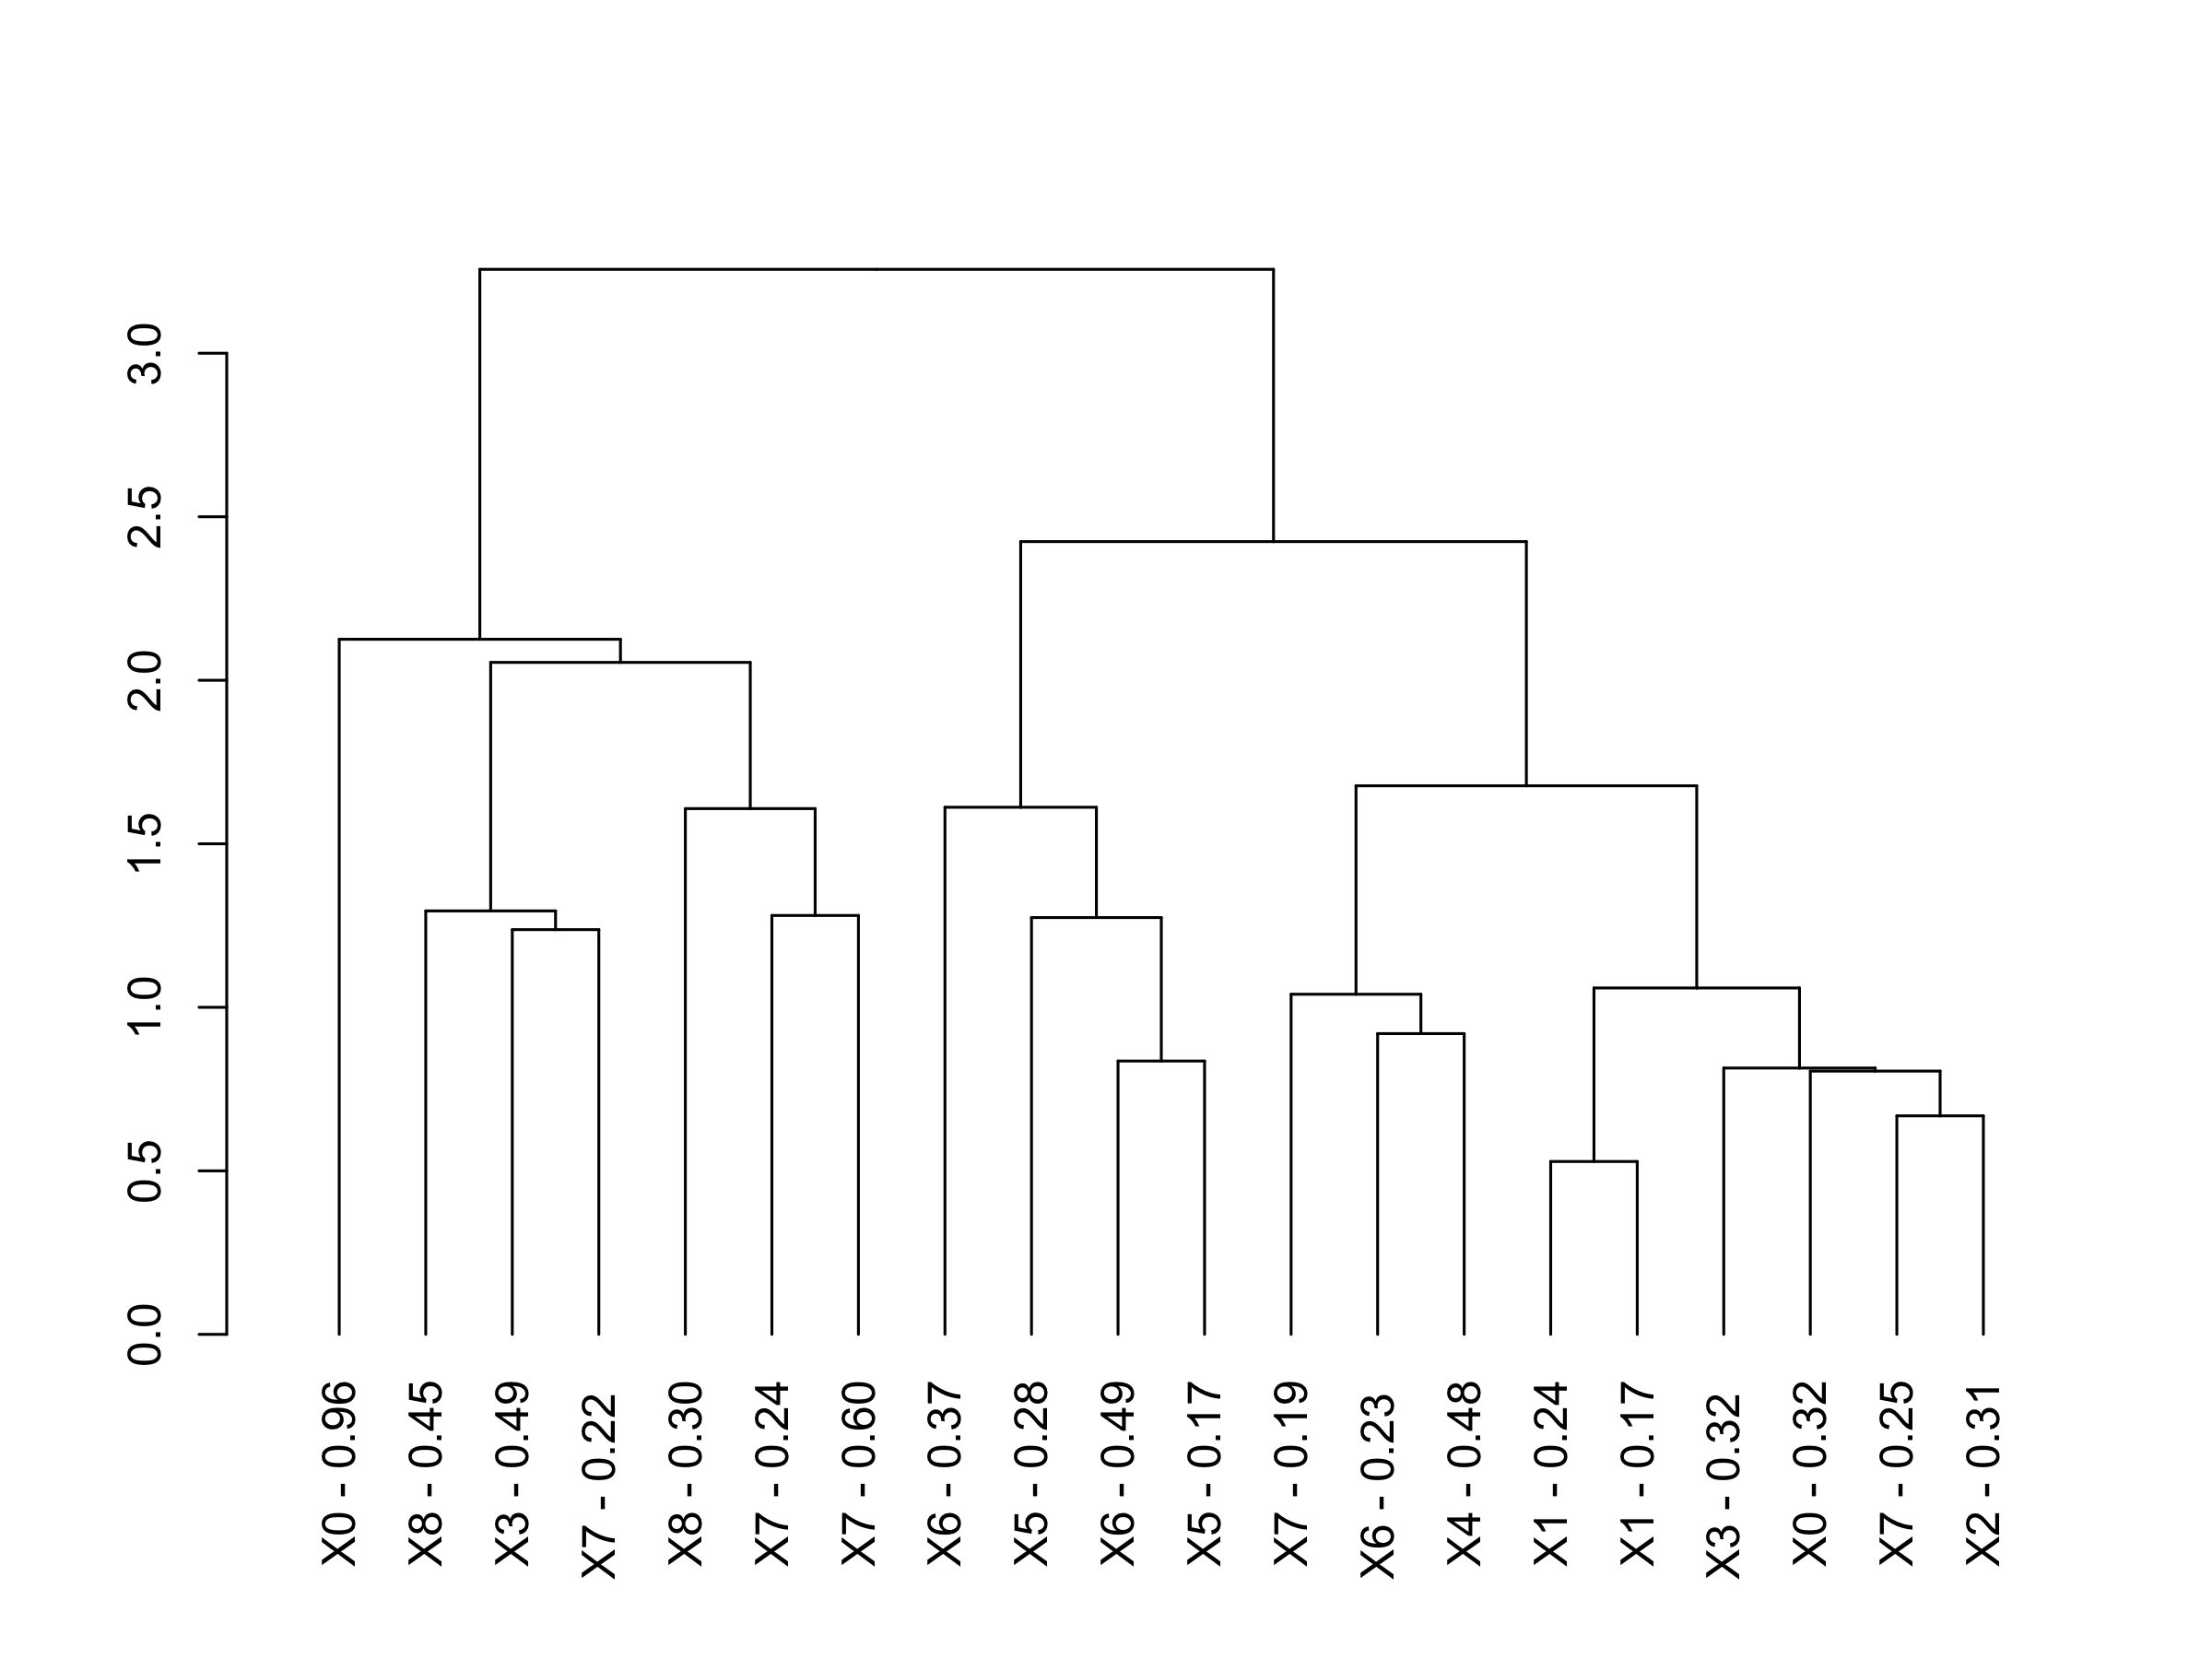
\includegraphics[width = 0.7\textwidth]{dendogram_data_class.png}
		 \caption{Dendrogram}
		 \label{fig:dendo}
\end{figure}																						

\begin{figure}[H]
\centering
\includegraphics[width = 0.7\textwidth]{confmatkNN-multiAll-sig15-k1-n40000.eps}
\caption{Confusion matrix}
\label{fig:confusionMatrixAll}
\end{figure}

In conclusion, in spite of the elbow method results,
30 clusters is too little for obtaining accurate classification results
with k-means clustering for the large dataset.
However, a general tendency towards large run time reduction was observed
using k-means clustering.
A brief analysis of hierarchical clustering results indicated
that a large number of clusters may be necessary
in order not to confuse certain similar digits, such as 2 and 7.
		
\end{document}